\documentclass{article}

\usepackage[utf8]{inputenc}
\usepackage{graphicx}
\usepackage{url}
\usepackage{color}
\usepackage{titlesec}
\usepackage{amsmath}
\usepackage{physics}
\usepackage{amsfonts}
\usepackage{subcaption}
\usepackage{booktabs}
\graphicspath{{../figures/}}

\title{paper draft: supersat}
\author{K. Latimer}
\date{Jan 13, 2020}

\begin{document}

\maketitle
\setcounter{section}{-1}

\section{Outline}
	\begin{enumerate}
		\item Introduction
		\item Based on WRF simulations, under what conditions is quasi-steady-state (QSS) approximation for supersaturation (SS) valid? [A: need to specify stringent enough LWC and vert wind vel cutoffs, only take points below freezing level, and include rain drops and ventilation corrections]
		\item Under above determined conditions, how do $SS_{QSS}$ distributions from WRF compare to those from experiments (CAIPEEX, HALO)? [A: statistically significant differences in distributions]
		\item Which variable contributes the most to the difference in $SS_{QSS}$ distributions? [A: ]
		\item Do environmental conditions allow for a fair comparison between simulation and experiment in these cases? [A: (pollution levels? vert wind vel / LWC distbns?)]
	\end{enumerate}

\section{Introduction}
introductory notes / lit review 

\section{Validity of QSS approximation for SS}
\begin{itemize}
	\item brief statement of quasi steady state formula 
	\item we see agreement between actual and QSS supersaturation under the conditions (see fig \ref{wrfvsqss}):
	\begin{itemize}
		\item T \textgreater  273K (we're not including ice in the theory)
		\item w \textgreater  2 m/s (reasonably strong updrafts)
		\item cloud LWC \textgreater  1e-4 g/g (in the convection core)
		\item including rain droplets and ventillation corrections
	\end{itemize}
	\item upon applying above filters, the distribution of $SS_{QSS}$ is shown in fig \ref{wrfssqsshist}.
\end{itemize}
\begin{figure}[ht]
	\centering
	\begin{subfigure}{0.7\textwidth}
		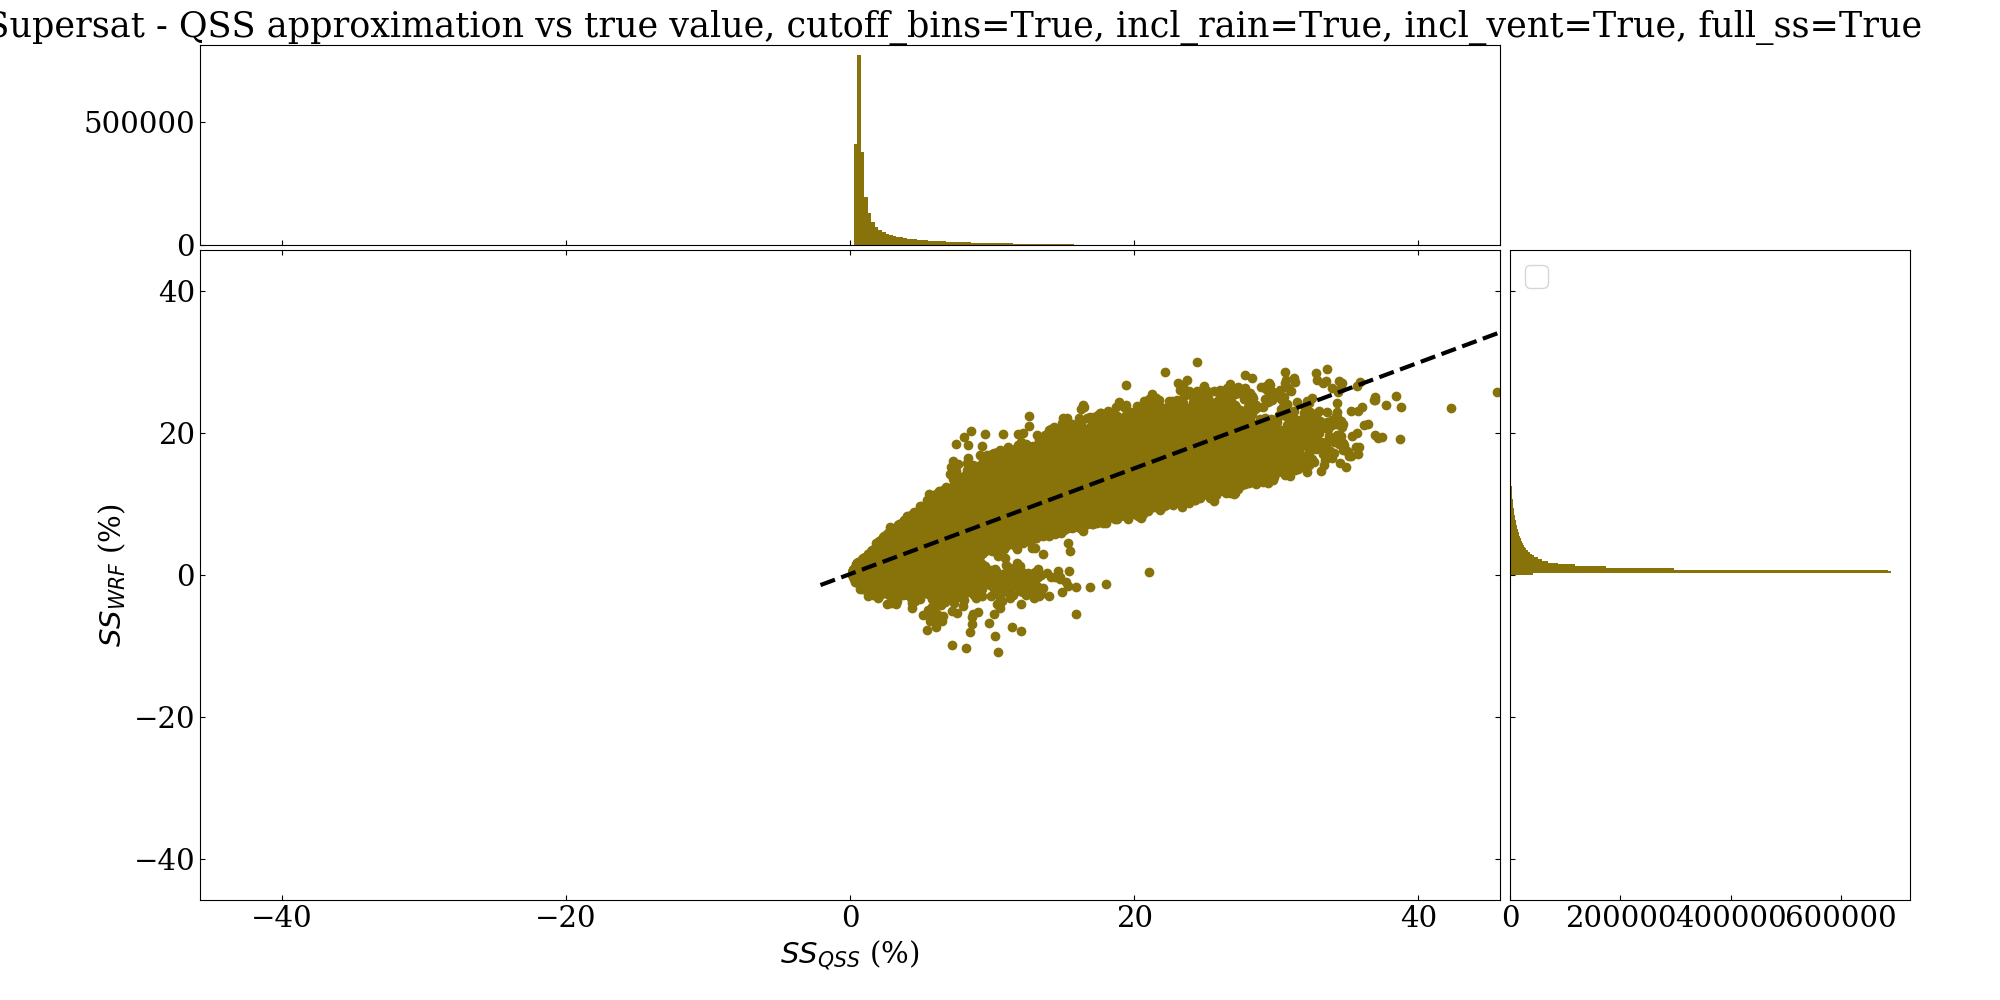
\includegraphics[width=\textwidth]{revmywrf/v12_fancy_ss_qss_vs_ss_wrf_Unpolluted_figure.png}
		\caption{Unpolluted case.}
		\label{wrfvsqssunpoll}
	\end{subfigure}
	\begin{subfigure}{0.7\textwidth}
		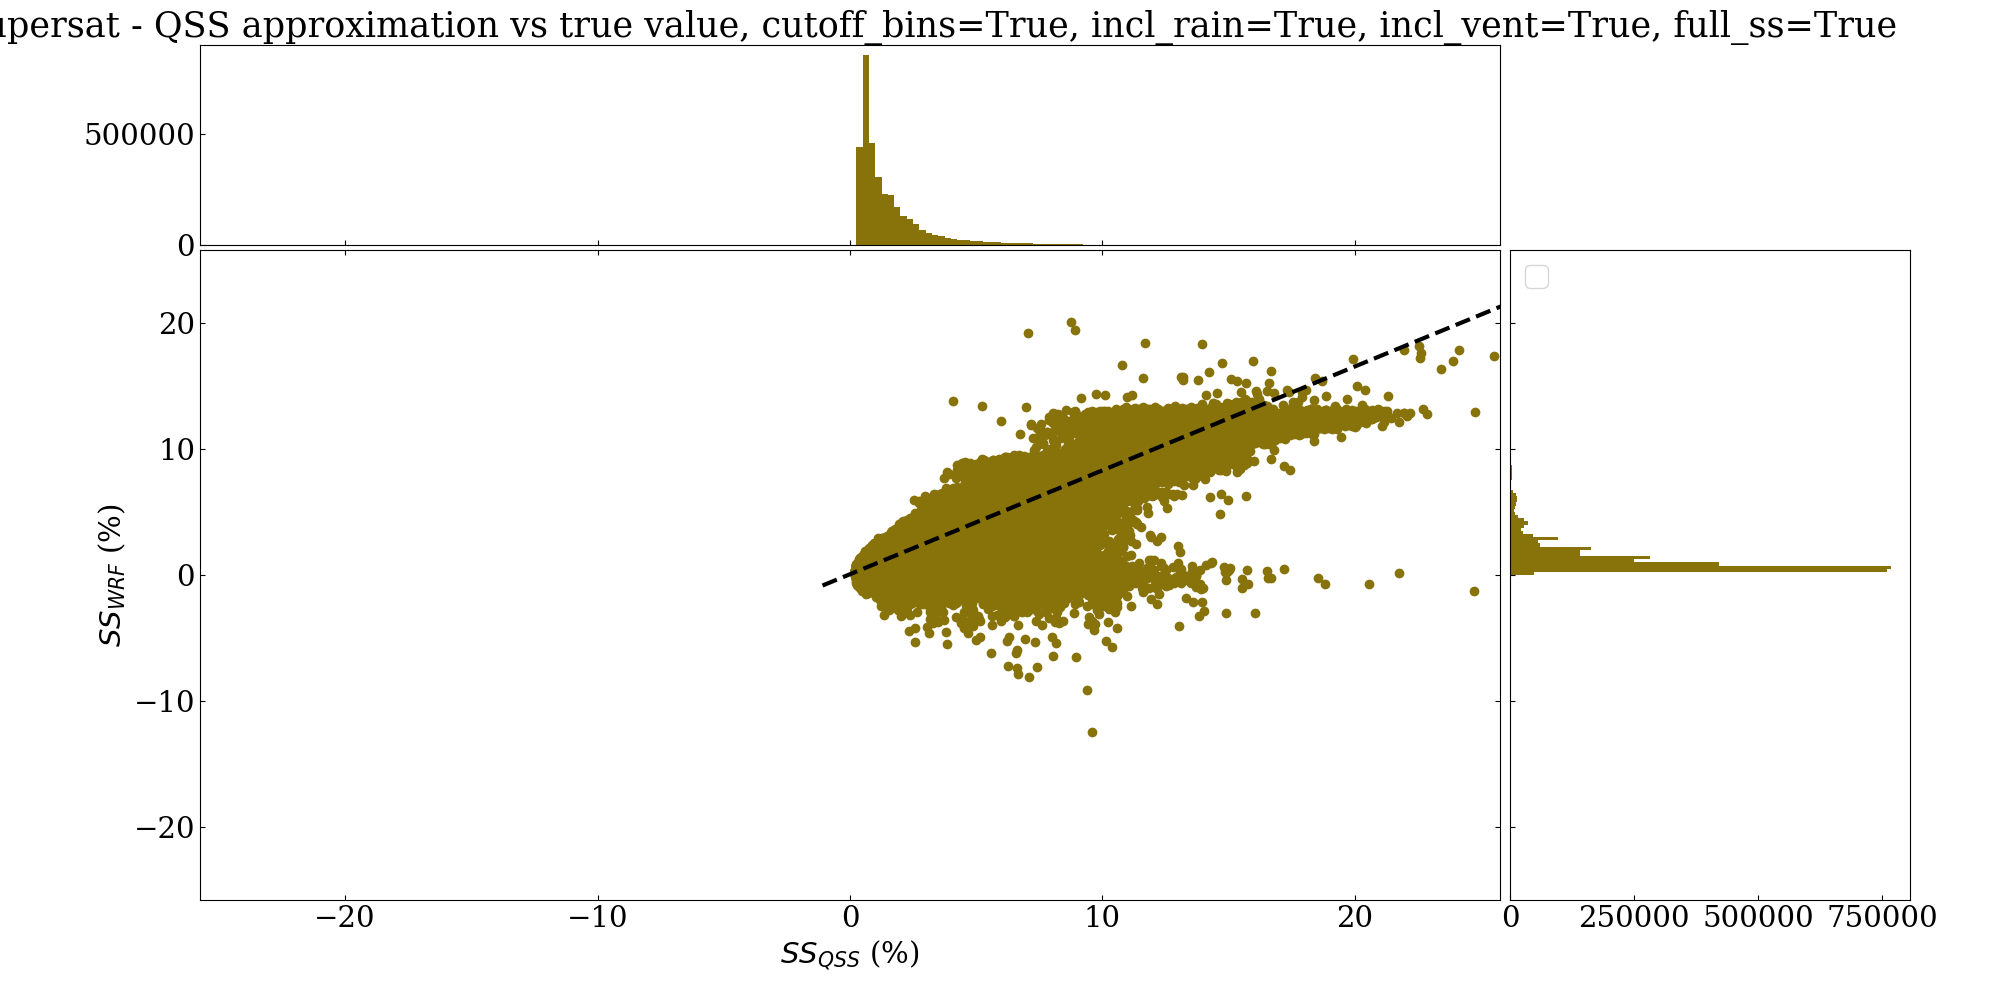
\includegraphics[width=\textwidth]{revmywrf/v12_fancy_ss_qss_vs_ss_wrf_Polluted_figure.png}
		\caption{Polluted case.}
		\label{wrfvsqsspoll}
	\end{subfigure}
	\caption{Actual ($SS_{WRF}$) vs predicted ($SS_{QSS}$) supersaturation. Histograms show the density of points along each axis.}
	\label{wrfvsqss}
\end{figure}
\begin{figure}[ht]
	\centering
	\begin{subfigure}{0.7\textwidth}
		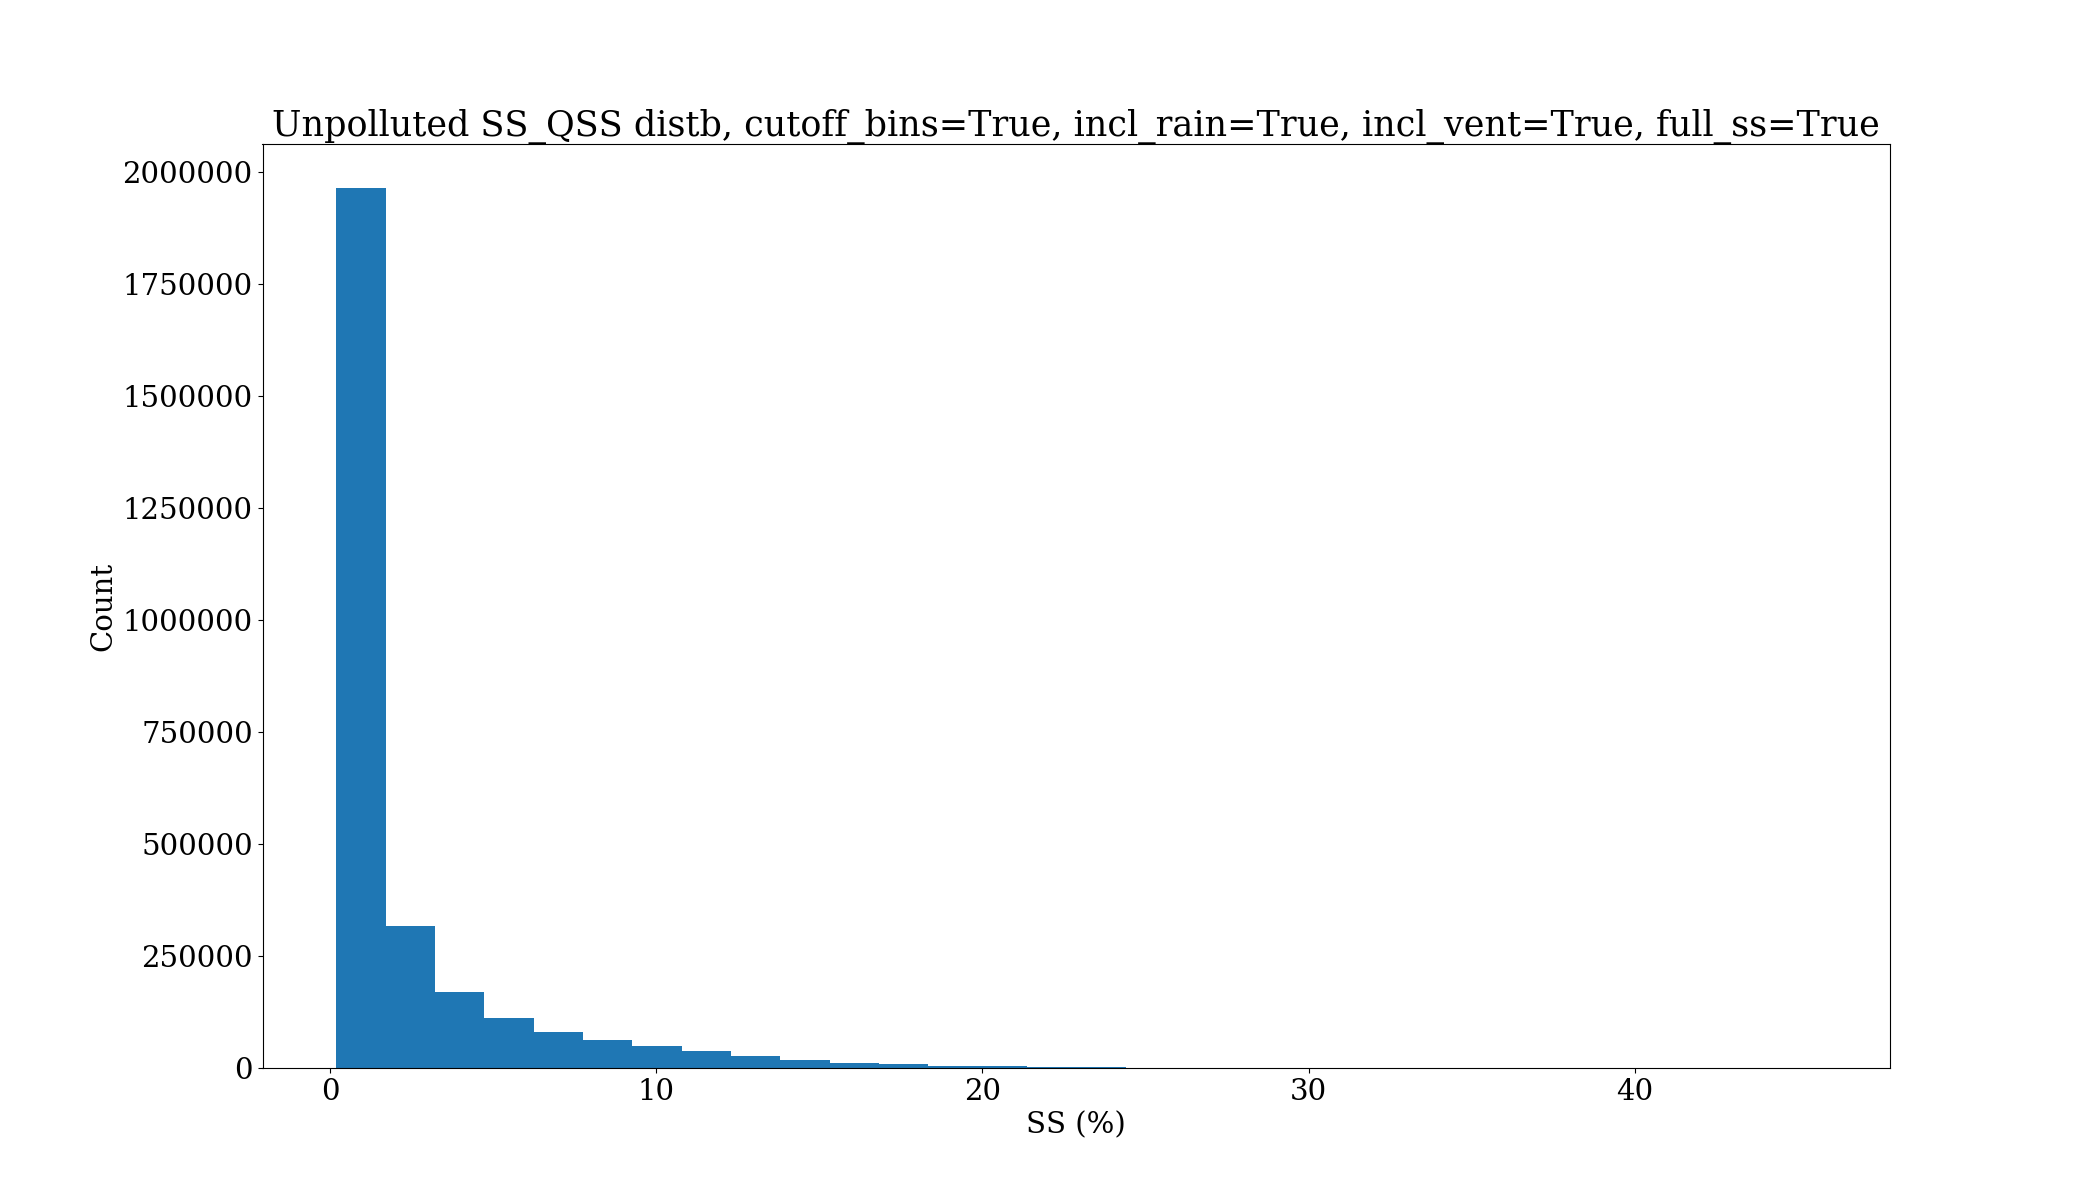
\includegraphics[width=\textwidth]{revmywrf/v12_ss_qss_hist_Unpolluted_figure.png}
		\caption{Unpolluted case.}
		\label{wrfssqsshistunpoll}
	\end{subfigure}
	\begin{subfigure}{0.7\textwidth}
		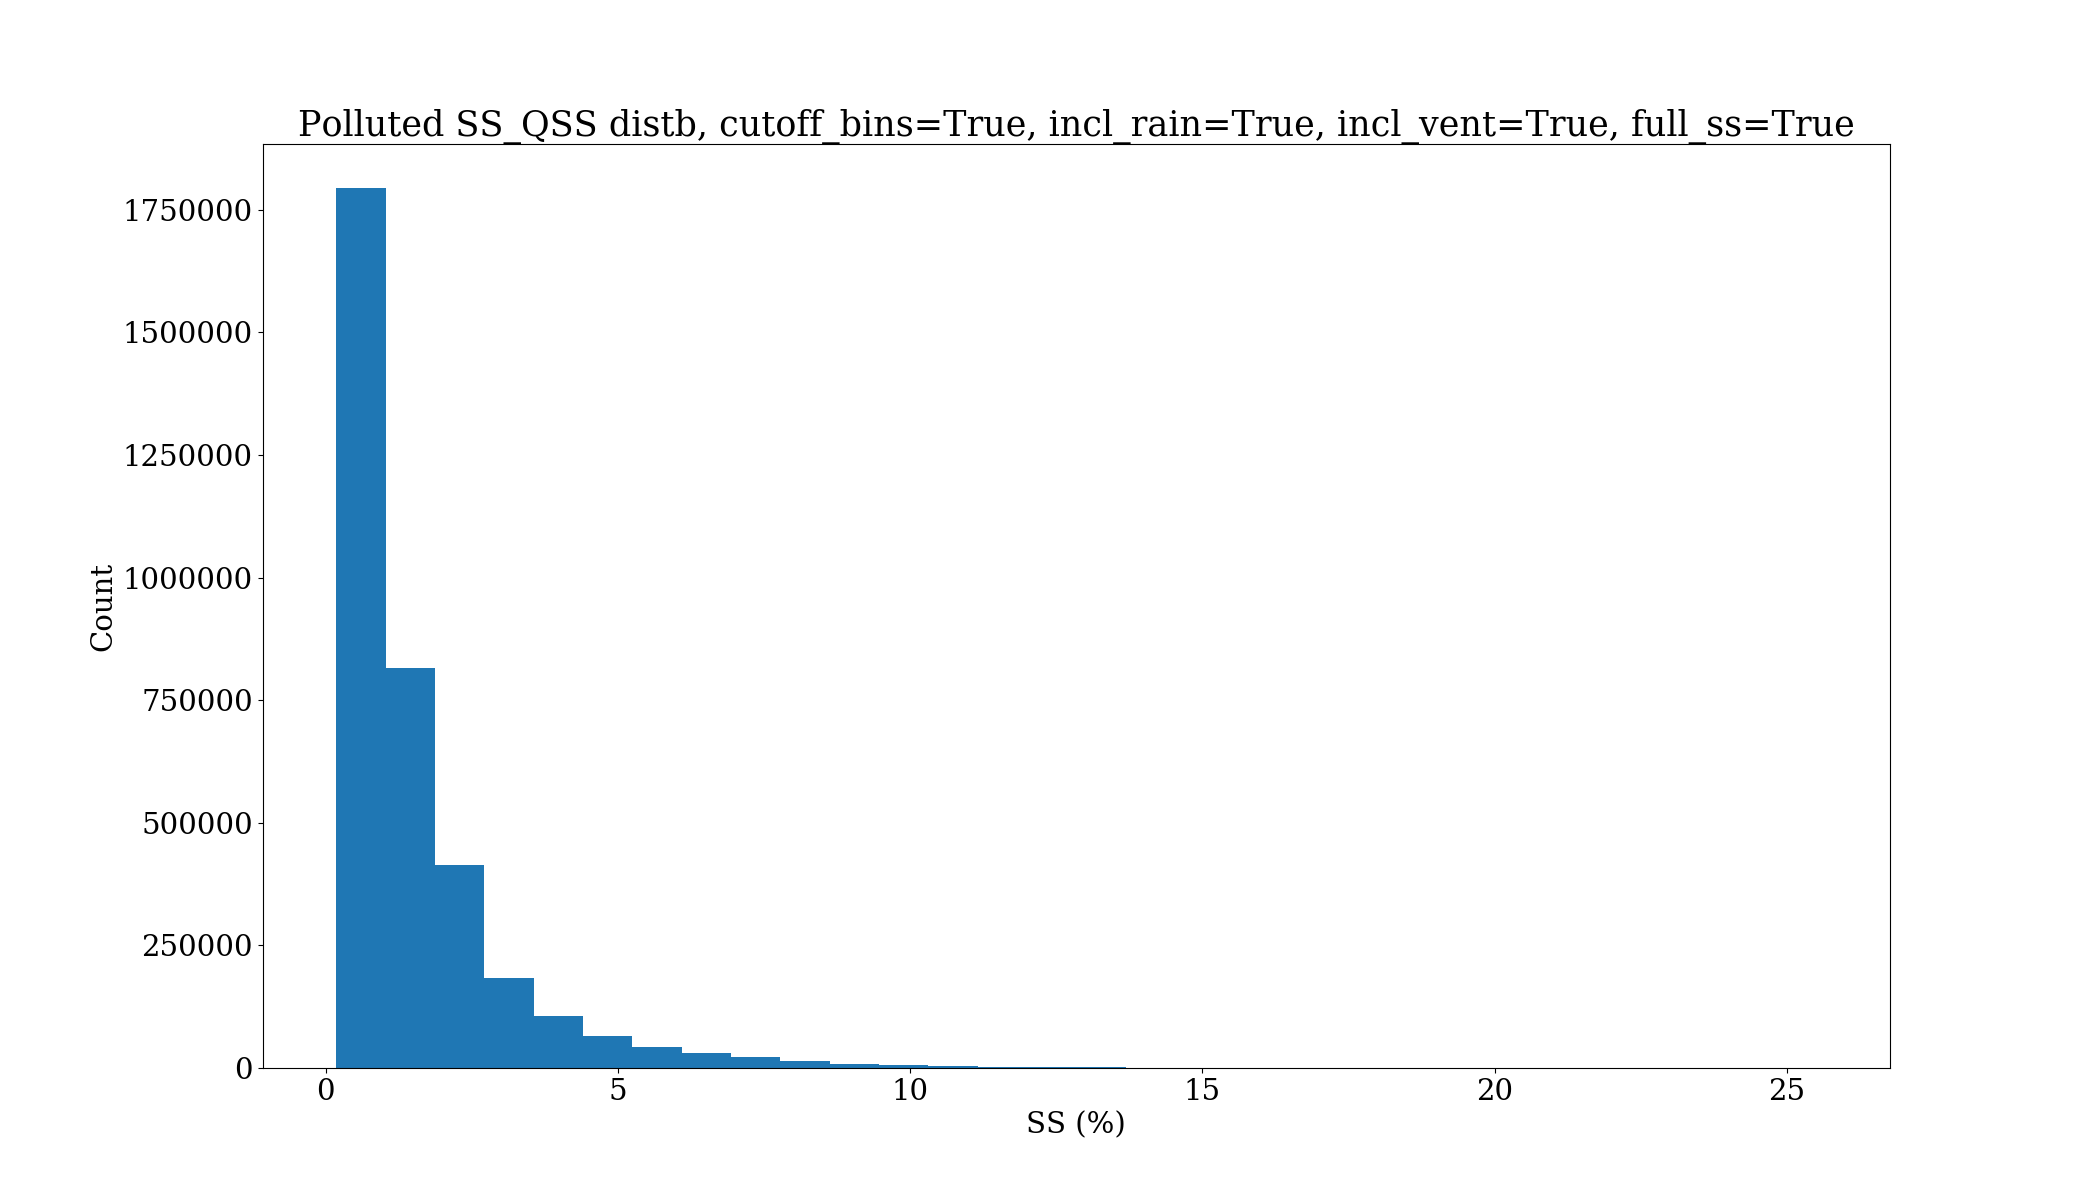
\includegraphics[width=\textwidth]{revmywrf/v12_ss_qss_hist_Polluted_figure.png}
		\caption{Polluted case.}
		\label{wrfssqsshistpoll}
	\end{subfigure}
	\caption{$SS_{WRF}$ distribution in WRF simulation using filtering criteria described in the text.}
	\label{wrfssqsshist}
\end{figure}

\clearpage
\newpage

\section{$SS_{QSS}$ distributions - simulation vs experiment}

\subsection{Distributions from field campaigns}
\begin{figure}[ht]
    \centering
    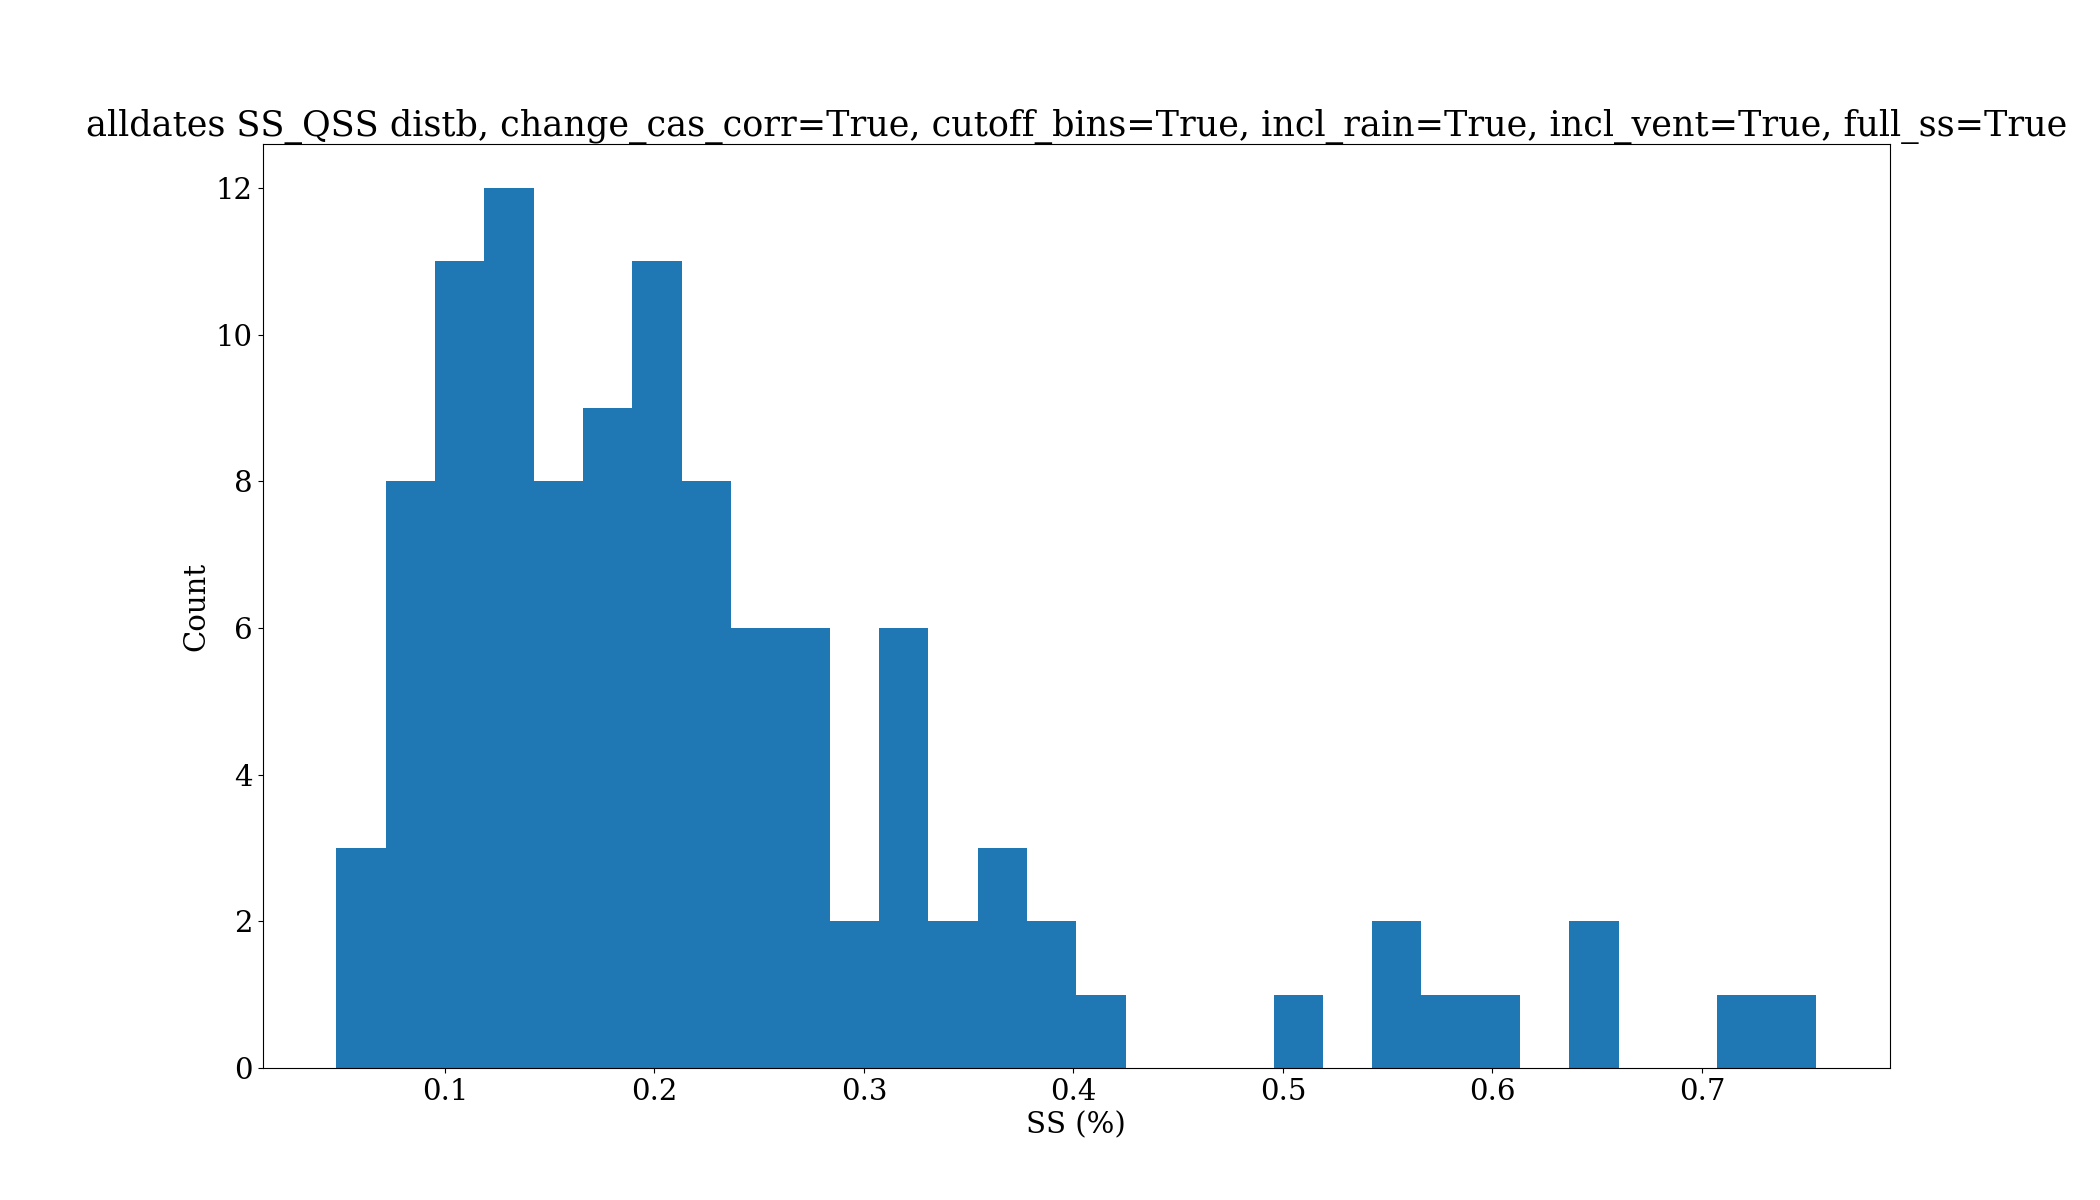
\includegraphics[width=9cm]{revhalo/v24_ss_qss_hist_cas_alldates_figure.png}
    \caption{Predicted ($SS_{QSS}$) supersaturation distribution from HALO field campaign (all flight dates). Using filtering criteria outlined in section 2.}
    \label{haloqsshist}
\end{figure}
\begin{figure}[ht]
    \centering
    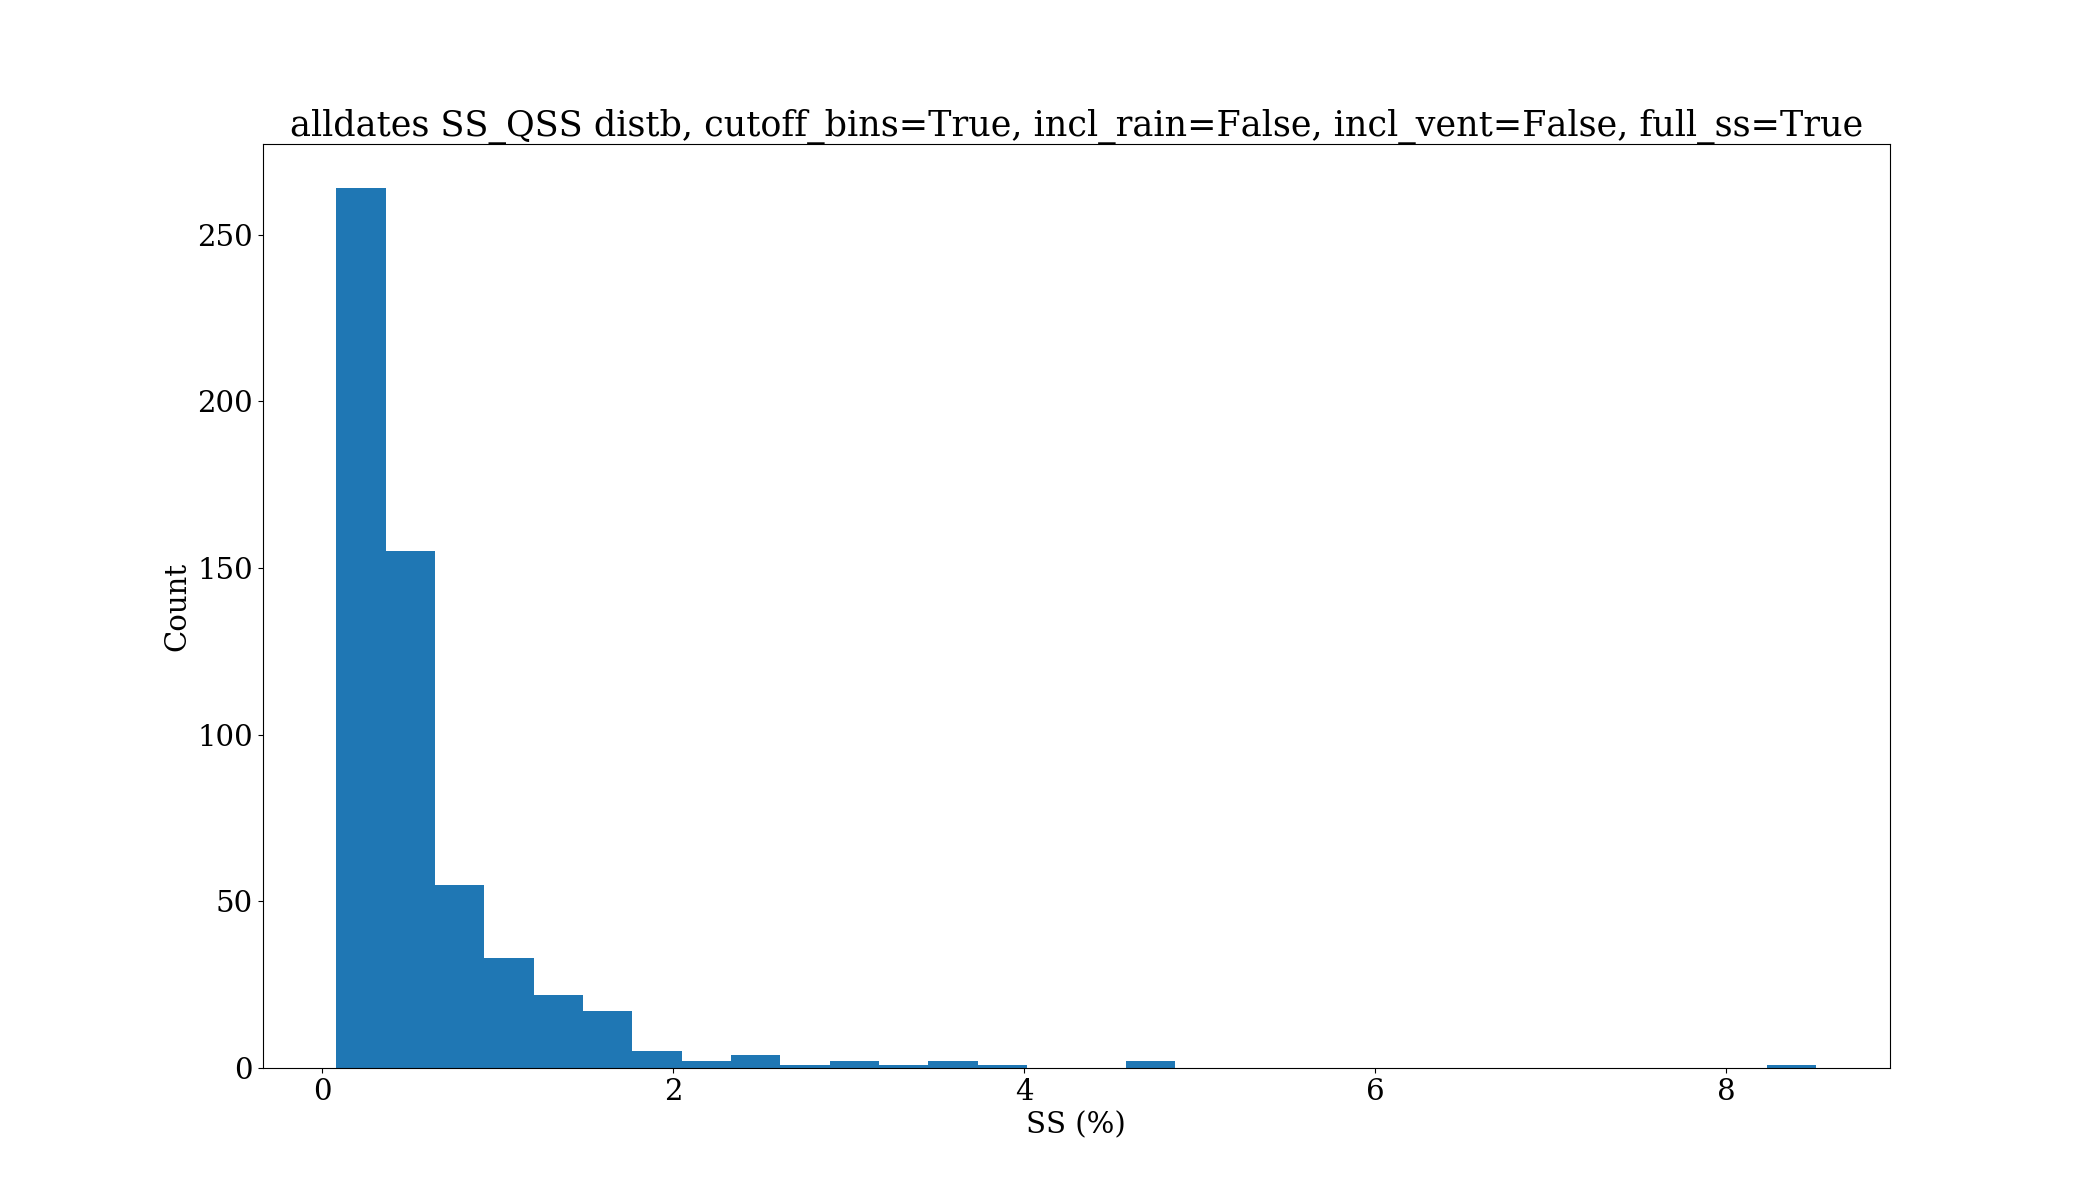
\includegraphics[width=9cm]{revcaipeex/v10_ss_qss_hist_alldates_figure.png}
    \caption{Predicted ($SS_{QSS}$) supersaturation distribution from CAIPEEX field campaign (all flight dates). Using filtering criteria outlined in section 2, but not including rain drops or ventilation corrections due to lack of data.}
    \label{caipeexqsshist}
\end{figure}

\subsection{Statistical analysis of supersaturation distributions}
\subsubsection{Null hypothesis}
Quasi-steady-state supersaturation values at selected sample of points from field campaigns are drawn from a ``true'' distribution like one of the ones from WRF. 
\subsubsection{Test}
Reduced chi-squared
\subsubsection{Details}
Since altitude shows non-negligible correlation with $SS_{QSS}$ in WRF data (Figure \ref{wrfssqssvsz}), we actually need to compare the experimental $SS_{QSS}$ distribution to an adjusted simulated distribution, to account for the differences in altitude distributions for sampled points in both datasets. Specifically:
\begin{equation}
\tilde\chi^2 = \frac{1}{d}\Big(\sum_{k} \frac{(\mathcal{O}_k - E_k)^2}{E_k}\Big),
\end{equation}
where $k$ labels discrete bins into which we group supersaturation values and,
\begin{align}
\mathcal{O}_k &= \text{# of measurements observed in bin $k$ (for all flight dates combined)}\nonumber\\
E_k &= \text{# of measurements observed in bin $k$ (under adjusted $SS_{QSS}$ distribution $P'_{sim}(SS_k)$)}\nonumber
\end{align}
The adjusted distribution is given by:
\begin{equation}
P'_{sim}(SS_k) = \sum_{j} P'_{sim}(z_j, SS_k),
\end{equation}
where,
\begin{equation}
P'_{sim}(z_j, SS_k) = \sum_{k''}\frac{P_{exp}(z_j, SS_{k''})P_{sim}(z_j, SS_k)}{\sum_{k'}P_{sim}(z_j, SS_{k'})}
\end{equation}

In this analysis, we had to use unequal bin sizes (i.e., group bins in the tail of the $SS_{QSS}$ distributions) in order to ensure $E'_k \geq 5$ and $n_{SS\hspace{0.2em}bins} \geq 4$ (the standard criteria for this statistical test). We set $d = n_{SS\hspace{0.2em}bins} - 2$ to account for the two choices of number of bins in the bivariate probability distributions $P(z_j, SS_k)$. \\

**NOTE** for now comparing CAIPEEX distributions to those from WRF output excluding rain drops since we don't have that data from CAIPEEX yet. Applies to all statistical analyses following.

\begin{figure}[ht]
	\centering
	\begin{subfigure}{0.7\textwidth}
		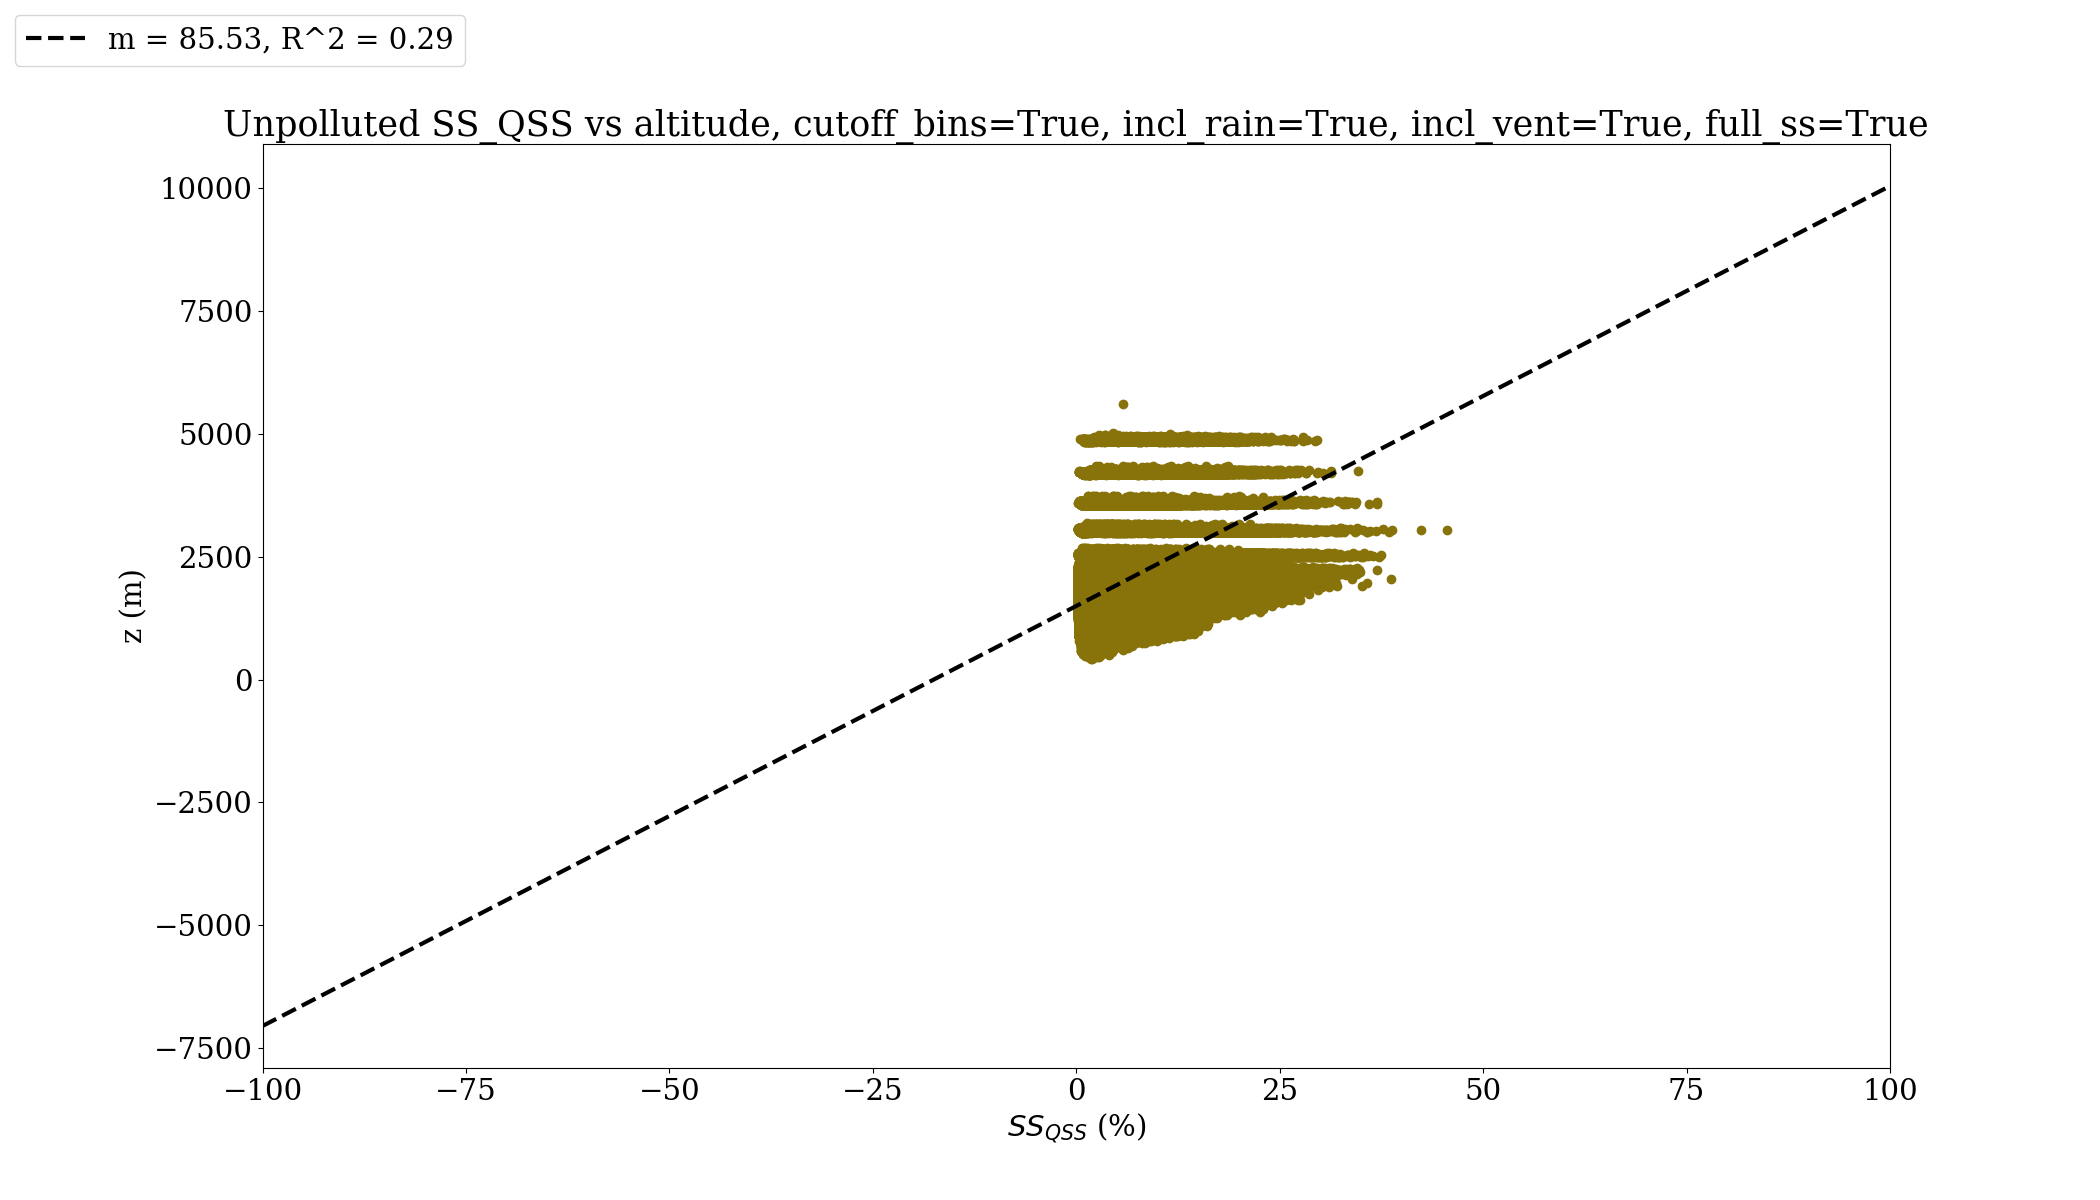
\includegraphics[width=\textwidth]{revmywrf/v12_ss_qss_vs_z_Unpolluted_figure.png}
		\caption{Unpolluted case.}
		\label{wrfssqssvszunpoll}
	\end{subfigure}
	\begin{subfigure}{0.7\textwidth}
		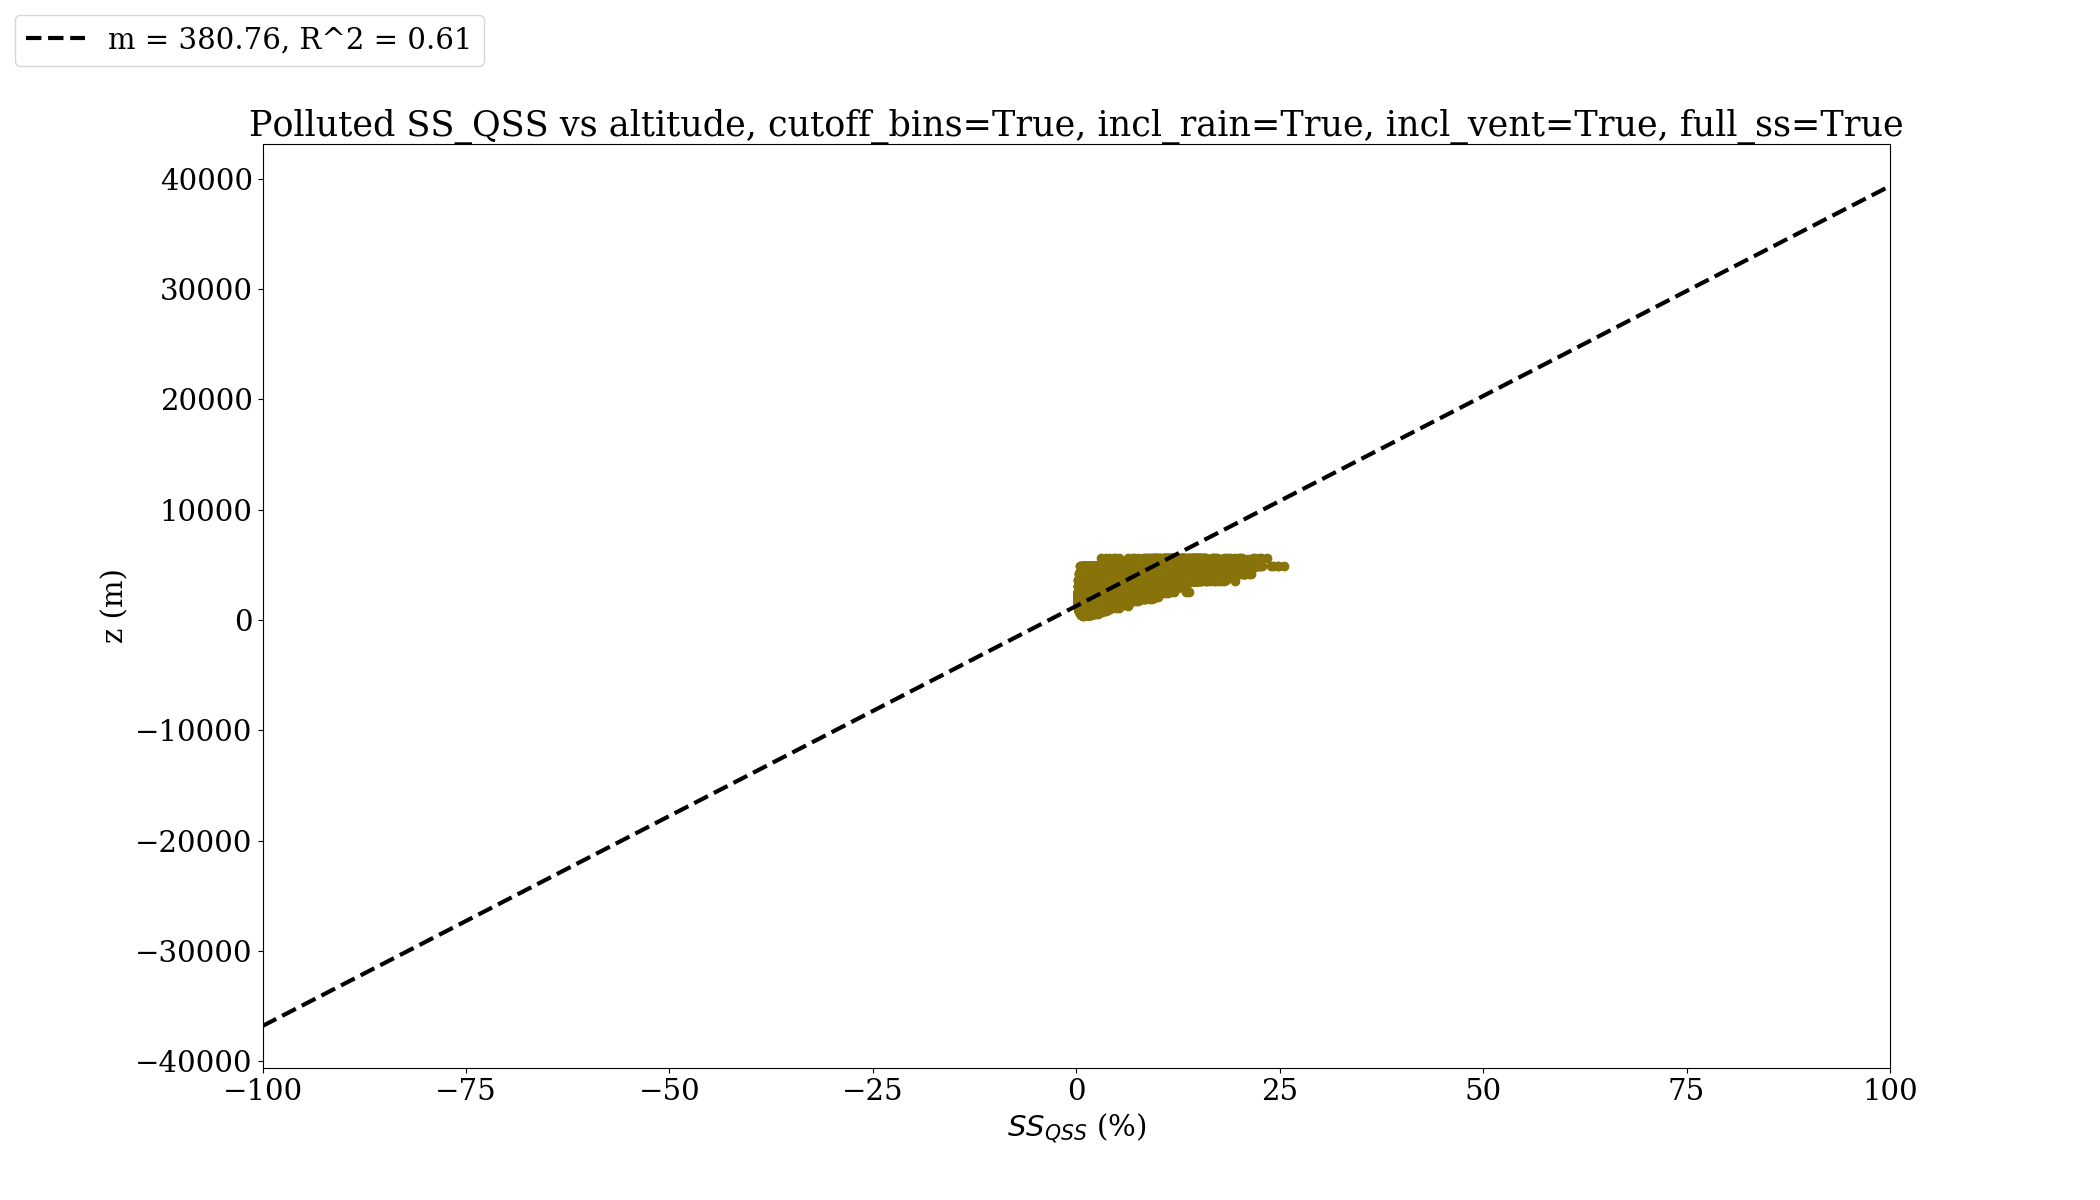
\includegraphics[width=\textwidth]{revmywrf/v12_ss_qss_vs_z_Polluted_figure.png}
		\caption{Polluted case.}
		\label{wrfssqssvszpoll}
	\end{subfigure}
	\caption{Scatter plots showing correlation between supersaturation as calculated in the QSS approximation and altitude in WRF simulations.}
	\label{wrfssqssvsz}
\end{figure}

\clearpage
\newpage

\subsubsection{Results}
\begin{table}[ht]
\centering
\begin{tabular}{@{}lllll@{}}
\toprule
\textbf{\# SS bins} & \textbf{\# z bins} & \textbf{$\tilde\chi^2$ (Polluted)} & \textbf{$\tilde\chi^2$ (Unpolluted)} & \textbf{$\tilde\chi^2_{0.990}$} \\ \midrule
4 & 10 & 37.24 & 25.01 & 4.61 \\
4 & 20 & 42.75 & 28.13 & 4.61 \\
4 & 30 & 44.58 & 32.28 & 4.61 \\
6 & 10 & 41.53 & 21.90 & 3.32 \\
6 & 20 & 51.20 & 25.77 & 3.32 \\
6 & 30 & 55.74 & 26.89 & 3.32 \\
8 & 10 & 45.96 & 17.46 & 2.80 \\
8 & 20 & 58.37 & 21.07 & 2.80 \\
8 / 7 & 30 & 64.83 & 26.44 & 2.80 / 3.10 \\ \bottomrule
\end{tabular}
\caption{Reduced chi squared test statistics for comparison of HALO $SS_{QSS}$ distribution to those in polluted and unpolluted cases of WRF simulation. Final column shows the critical value of $\tilde\chi^2$, above which we reject the null hypothesis at the 99\% confidence level. Entries separated by forward slash indicate different number of SS bins used to compare to polluted and unpolluted cases.}
\label{halochisqtable}
\end{table}
\begin{table}[ht]
\centering
\begin{tabular}{@{}lllll@{}}
\toprule
\textbf{\# SS bins} & \textbf{\# z bins} & \textbf{$\tilde\chi^2$ (Polluted)} & \textbf{$\tilde\chi^2$ (Unpolluted)} & \textbf{$\tilde\chi^2_{0.990}$} \\ \midrule
4 & 10 & 114.91 & 169.54 & 4.61 \\
4 & 20 & 128.36 & 212.82 & 4.61 \\
4 & 30 & 141.68 & 179.69 & 4.61 \\
6 & 10 & 120.17 & 152.94 & 3.32 \\
5 / 6 & 20 & 176.79 & 170.97 & 3.78 / 3.32 \\
6 & 30 & 140.27 & 164.95 & 3.32 \\
7 / 8 & 10 & 149.86 & 136.48 & 3.10 / 2.80 \\
7 & 20 & 160.19 & 173.21 & 3.10 \\
7 & 30 & 165.58 & 182.97 & 3.10 \\ \bottomrule
\end{tabular}
\caption{Reduced chi squared test statistics for comparison of CAIPEEX (2009 flights) $SS_{QSS}$ distribution to those in polluted and unpolluted cases of WRF simulation. Final column shows the critical value of $\tilde\chi^2$, above which we reject the null hypothesis at the 99\% confidence level. Entries separated by forward slash indicate different number of SS bins used to compare to polluted and unpolluted cases.}
\label{caipeexchisqtable}
\end{table}

\clearpage
\newpage

\subsubsection{Comments}
\begin{itemize}
	\item For HALO: test statistics do show considerable sensitivity to binning arrangement, but are so far above the critical values that this seems largely irrelevant. We reject the null hypothesis in this case with very high (quantify?) certainty.
	\item For CAIPEEX: ditto. Chi-squared values are larger for this dataset because the sample size is higher ($\approx$600 points cf $\approx$100 in HALO)
\end{itemize}

\section{Causes of discrepancies between $SS_{QSS}$ distributions (sim vs exp)}
- under above filtering criteria: meanr distbs for wrf (FIG), halo (FIG) and caipeex (FIG)
- stat analysis meanr 
- under above filtering criteria: nconc distbs for wrf (FIG), halo (FIG) and caipeex (FIG)
- stat analysis nconc 
- under above filtering criteria: w distbs for wrf (FIG), halo (FIG) and caipeex (FIG)
- stat analysis w 

Up to temperature-dependent prefactors we have:
\begin{equation}
SS_{QSS} \sim \frac{w}{\langle f(r)\cdot r \rangle n},
\end{equation}
where $w$ is vertical wind velocity, $f(r)$ is ventilation factor, $r$ is water drop radius, $n$ is water drop number concentration, and $\langle y(r) \rangle$ denotes the average of function $y$ over the radial domain of the given drop size distribution. We compare the distributions of these three quantities in simulation vs experiment below in the same manner as for supersaturation in the previous section.

\subsection{Mean radius (with ventilation correction)}

\begin{figure}[ht]
	\centering
	\begin{subfigure}{0.7\textwidth}
		\includegraphics[width=\textwidth]{revmywrf/v9_meanr_hist_Unpolluted_figure.png}
		\caption{Unpolluted case.}
		\label{wrfmeanrhistunpoll}
	\end{subfigure}
	\begin{subfigure}{0.7\textwidth}
		\includegraphics[width=\textwidth]{revmywrf/v9_meanr_hist_Polluted_figure.png}
		\caption{Polluted case.}
		\label{wrfmeanrhistpoll}
	\end{subfigure}
	\caption{Mean radius (ventilation corrected) distribution in WRF simulation using filtering criteria described in the text.}
	\label{wrfmeanrhist}
\end{figure}
\begin{figure}[ht]
    \centering
    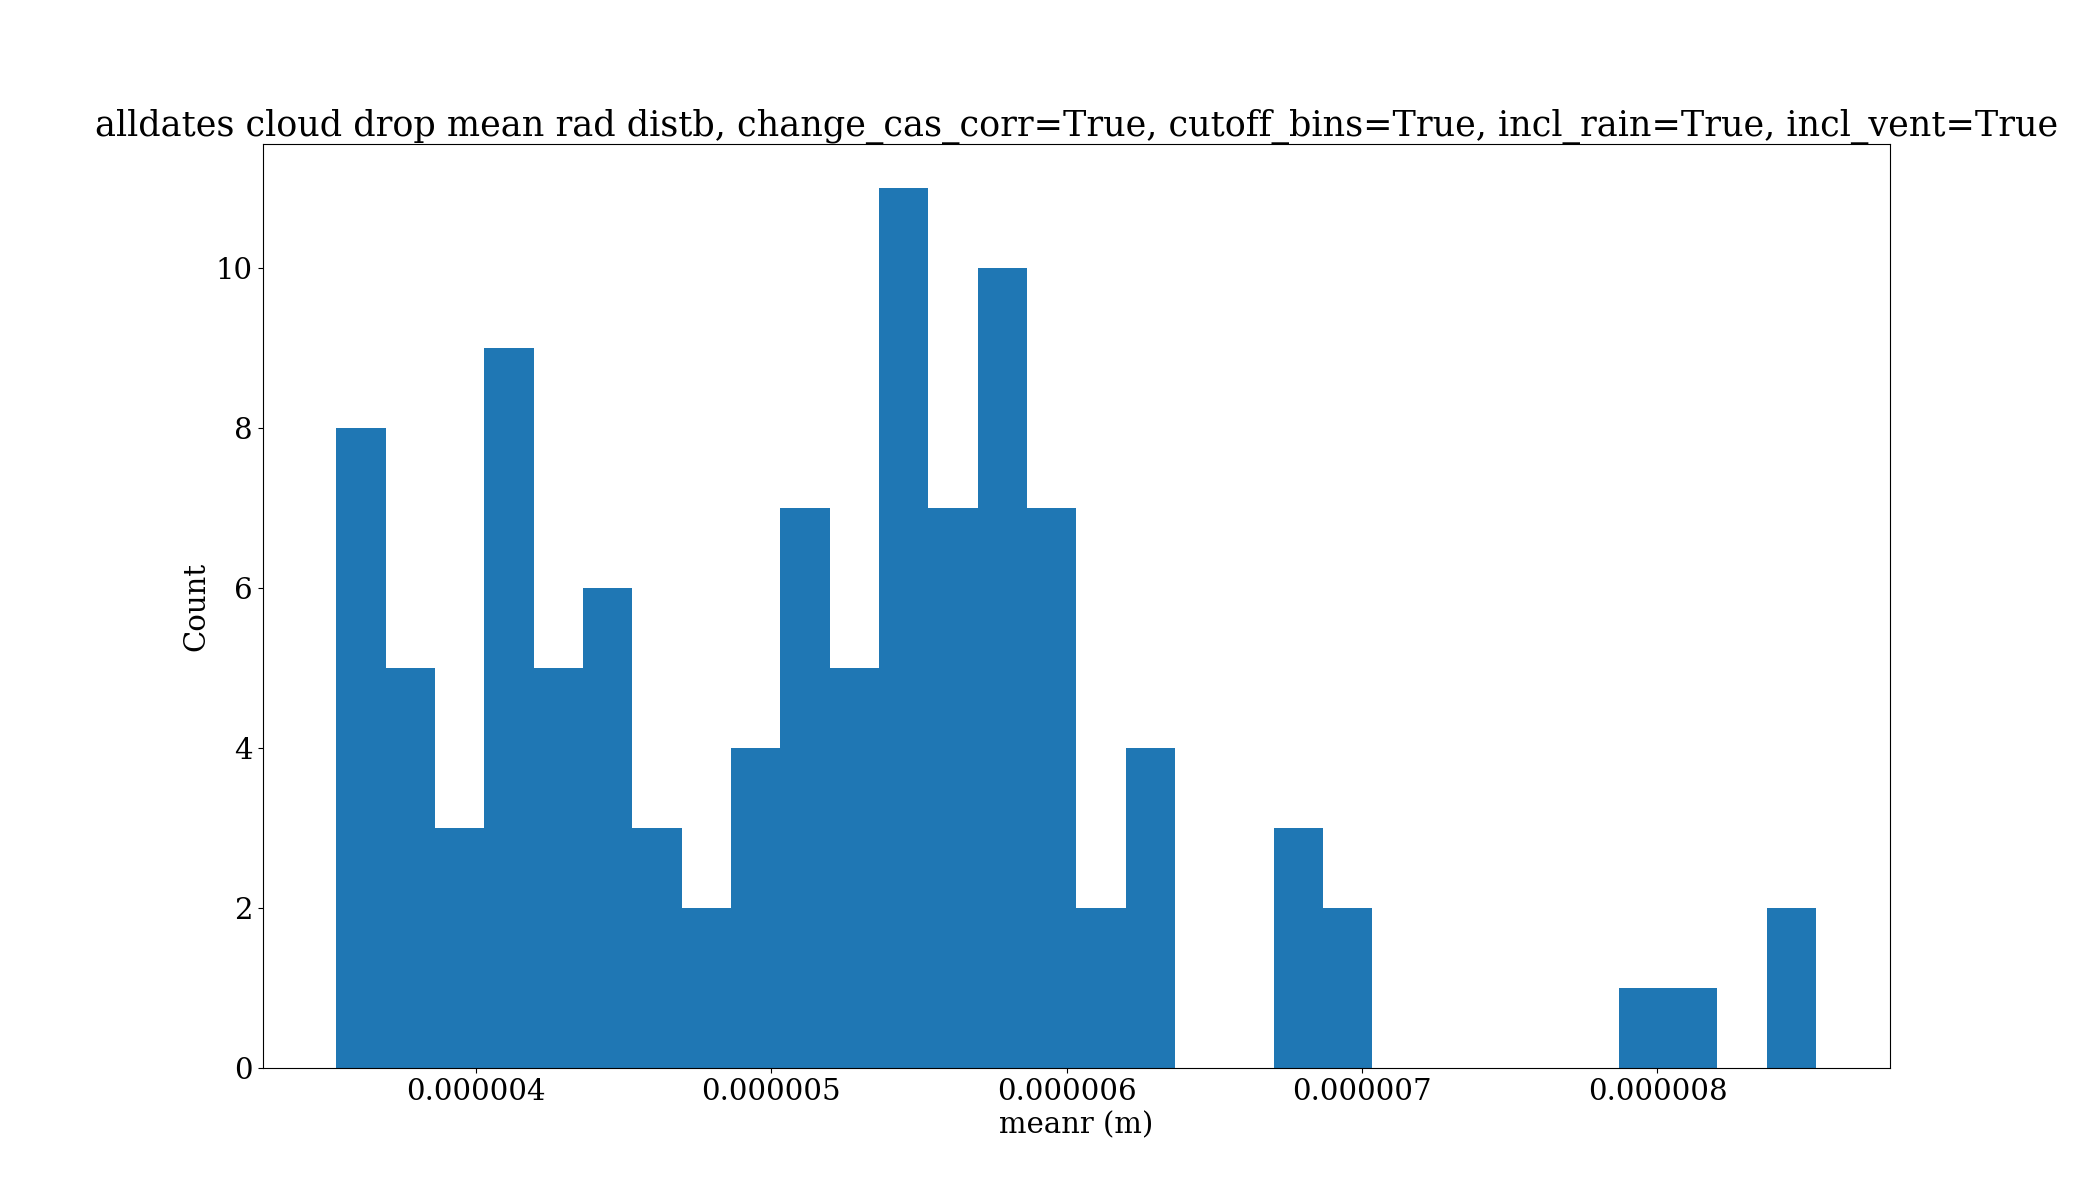
\includegraphics[width=9cm]{revhalo/v24_meanr_hist_cas_alldates_figure.png}
    \caption{Mean radius (with ventilation corrections) distribution from HALO field campaign (all flight dates). Using filtering criteria outlined in section 2.}
    \label{haloqsshist}
\end{figure}
\begin{figure}[ht]
    \centering
    \includegraphics[width=9cm]{revcaipeex/v10_meanr_hist_alldates_figure.png}
    \caption{Mean radius distribution from CAIPEEX field campaign (all flight dates). Using filtering criteria outlined in section 2, but not including rain drops or ventilation corrections due to lack of data.}
    \label{caipeexqsshist}
\end{figure}

\subsection{Number concentration}

\begin{figure}[ht]
	\centering
	\begin{subfigure}{0.7\textwidth}
		\includegraphics[width=\textwidth]{revmywrf/v9_nconc_hist_Unpolluted_figure.png}
		\caption{Unpolluted case.}
		\label{wrfnconchistunpoll}
	\end{subfigure}
	\begin{subfigure}{0.7\textwidth}
		\includegraphics[width=\textwidth]{revmywrf/v9_nconc_hist_Polluted_figure.png}
		\caption{Polluted case.}
		\label{wrfnconchistpoll}
	\end{subfigure}
	\caption{Number concentration distribution in WRF simulation using filtering criteria described in the text.}
	\label{wrfnconchist}
\end{figure}
\begin{figure}[ht]
    \centering
    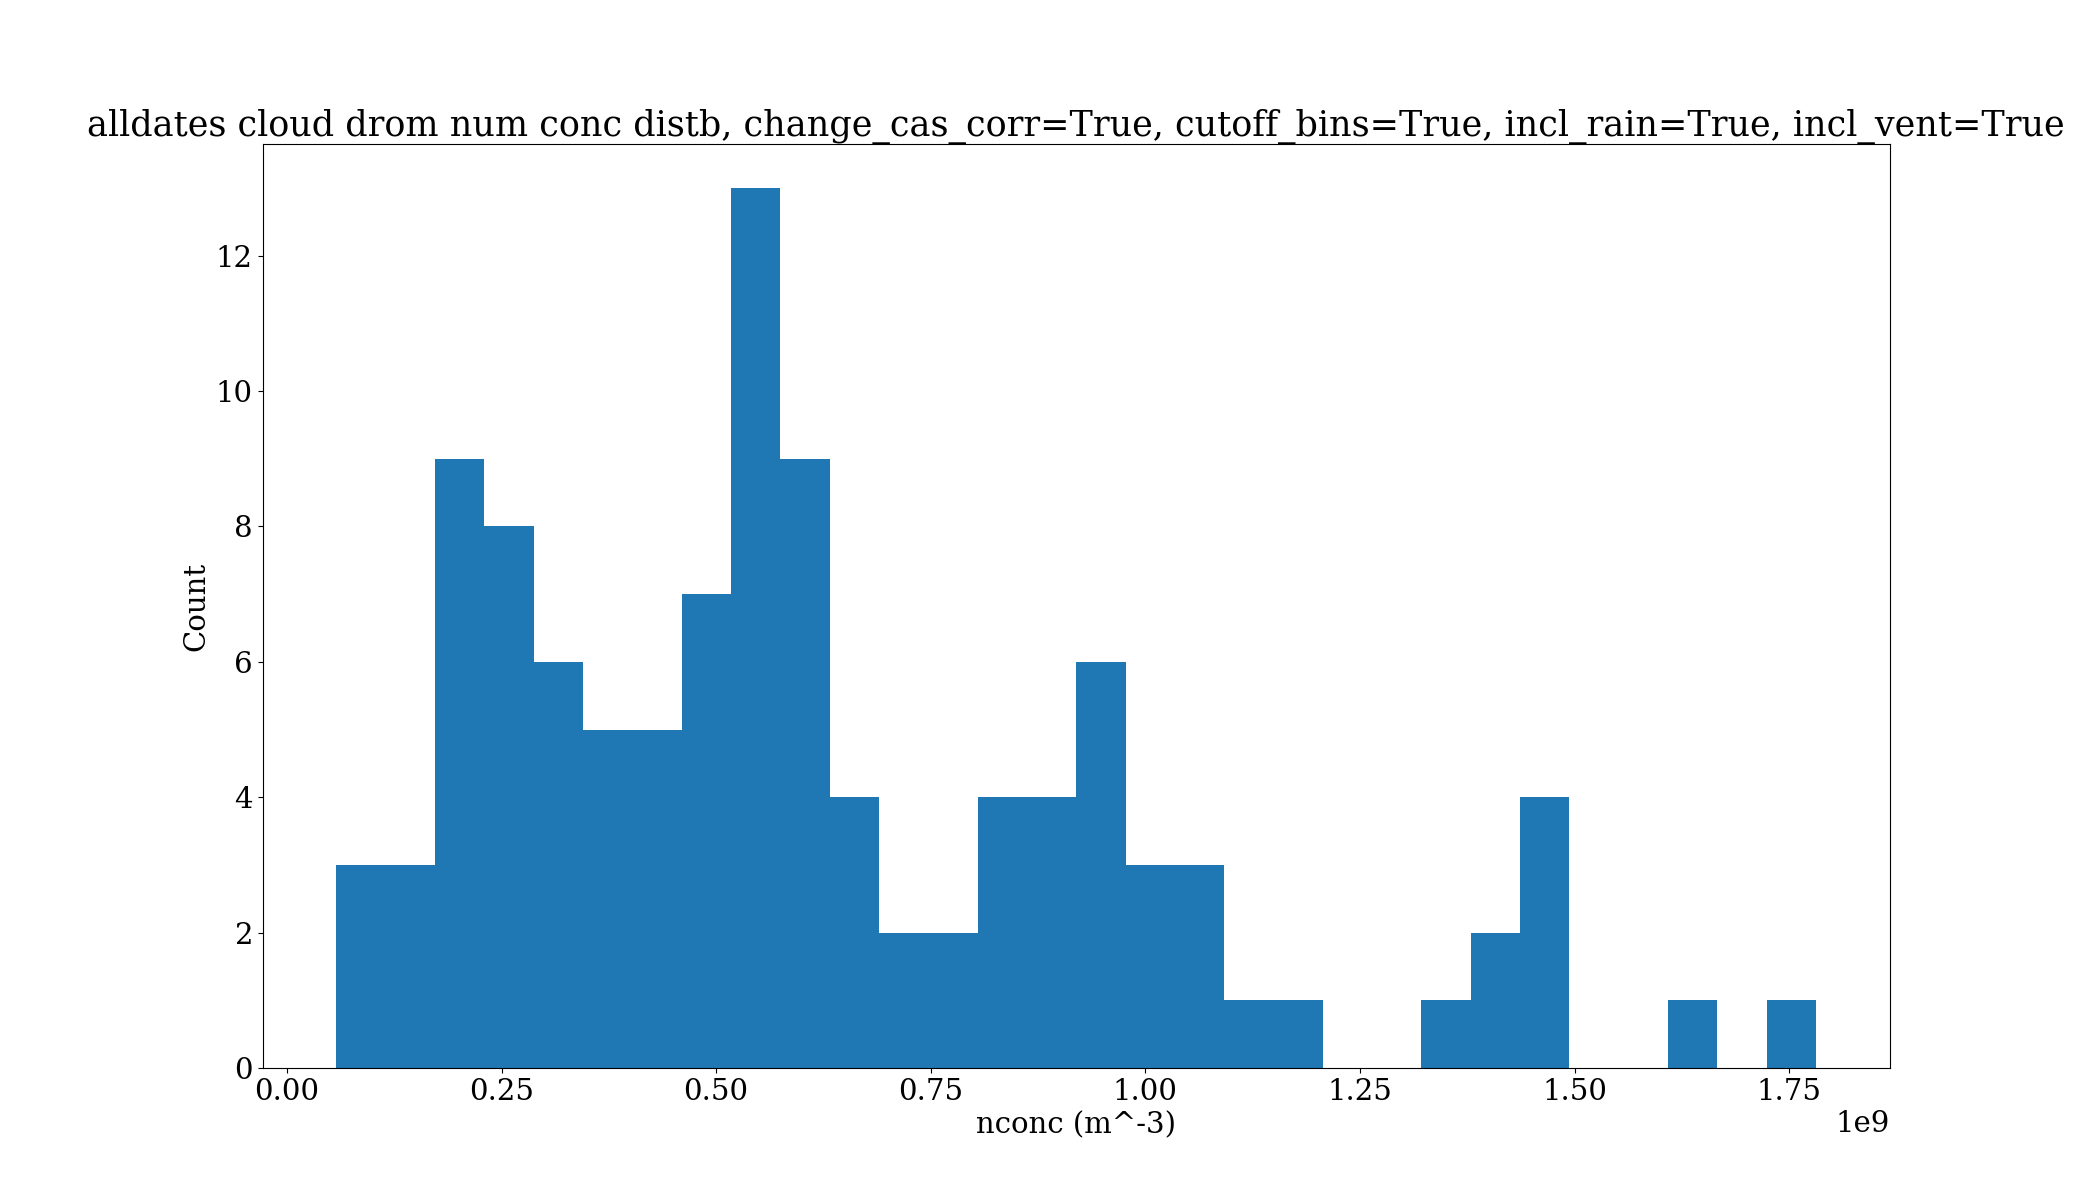
\includegraphics[width=9cm]{revhalo/v24_nconc_hist_cas_alldates_figure.png}
    \caption{Number concentration distribution from HALO field campaign (all flight dates). Using filtering criteria outlined in section 2.}
    \label{haloqsshist}
\end{figure}
\begin{figure}[ht]
    \centering
    \includegraphics[width=9cm]{revcaipeex/v10_nconc_hist_alldates_figure.png}
    \caption{Number concentration distribution from CAIPEEX field campaign (all flight dates). Using filtering criteria outlined in section 2, but not including rain drops or ventilation corrections due to lack of data.}
    \label{caipeexqsshist}
\end{figure}

\subsection{Vertical wind velocity}

\begin{figure}[ht]
	\centering
	\begin{subfigure}{0.7\textwidth}
		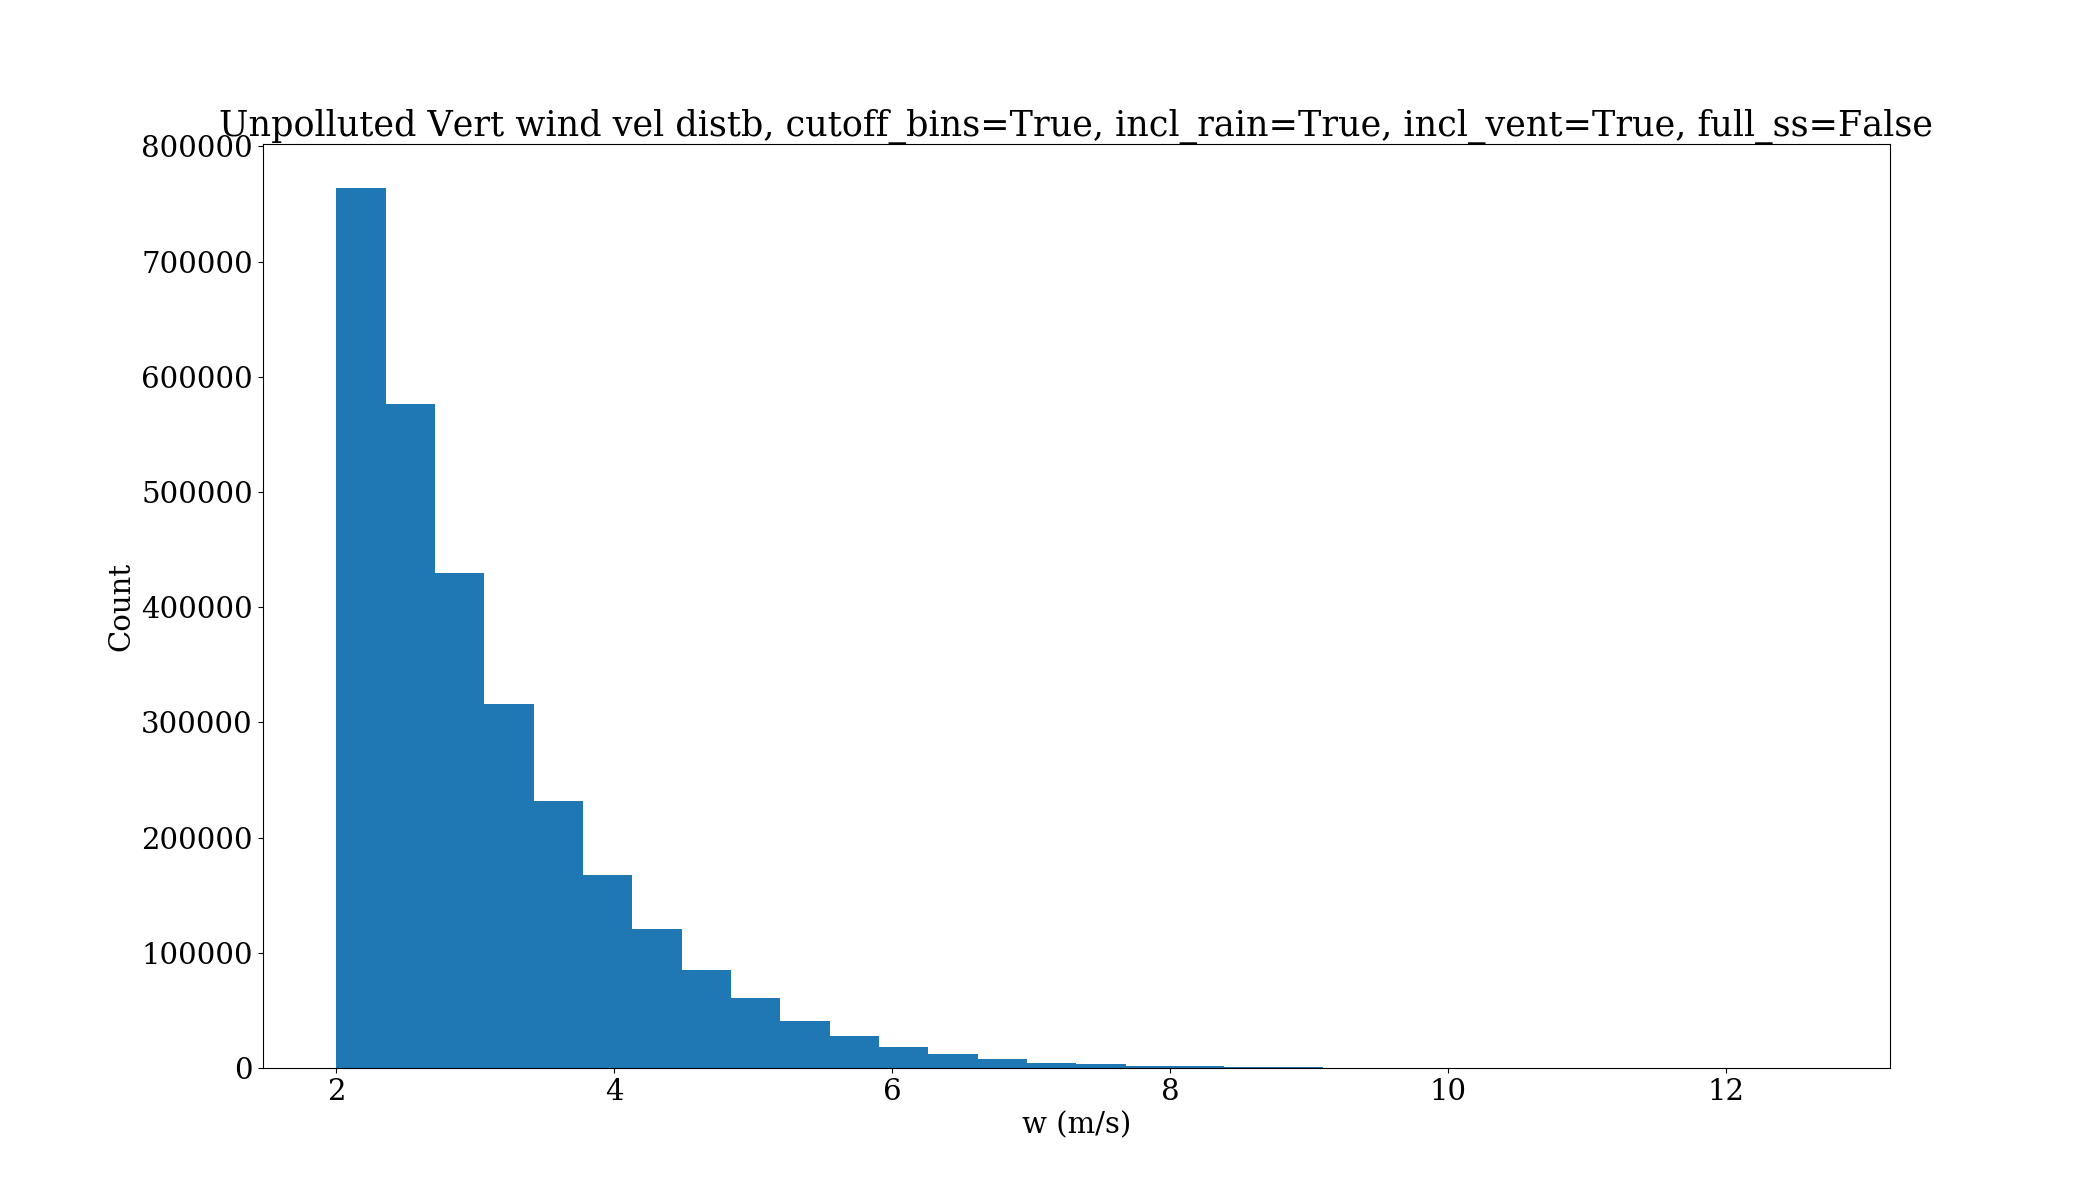
\includegraphics[width=\textwidth]{revmywrf/v9_w_hist_Unpolluted_figure.png}
		\caption{Unpolluted case.}
		\label{wrfwhistunpoll}
	\end{subfigure}
	\begin{subfigure}{0.7\textwidth}
		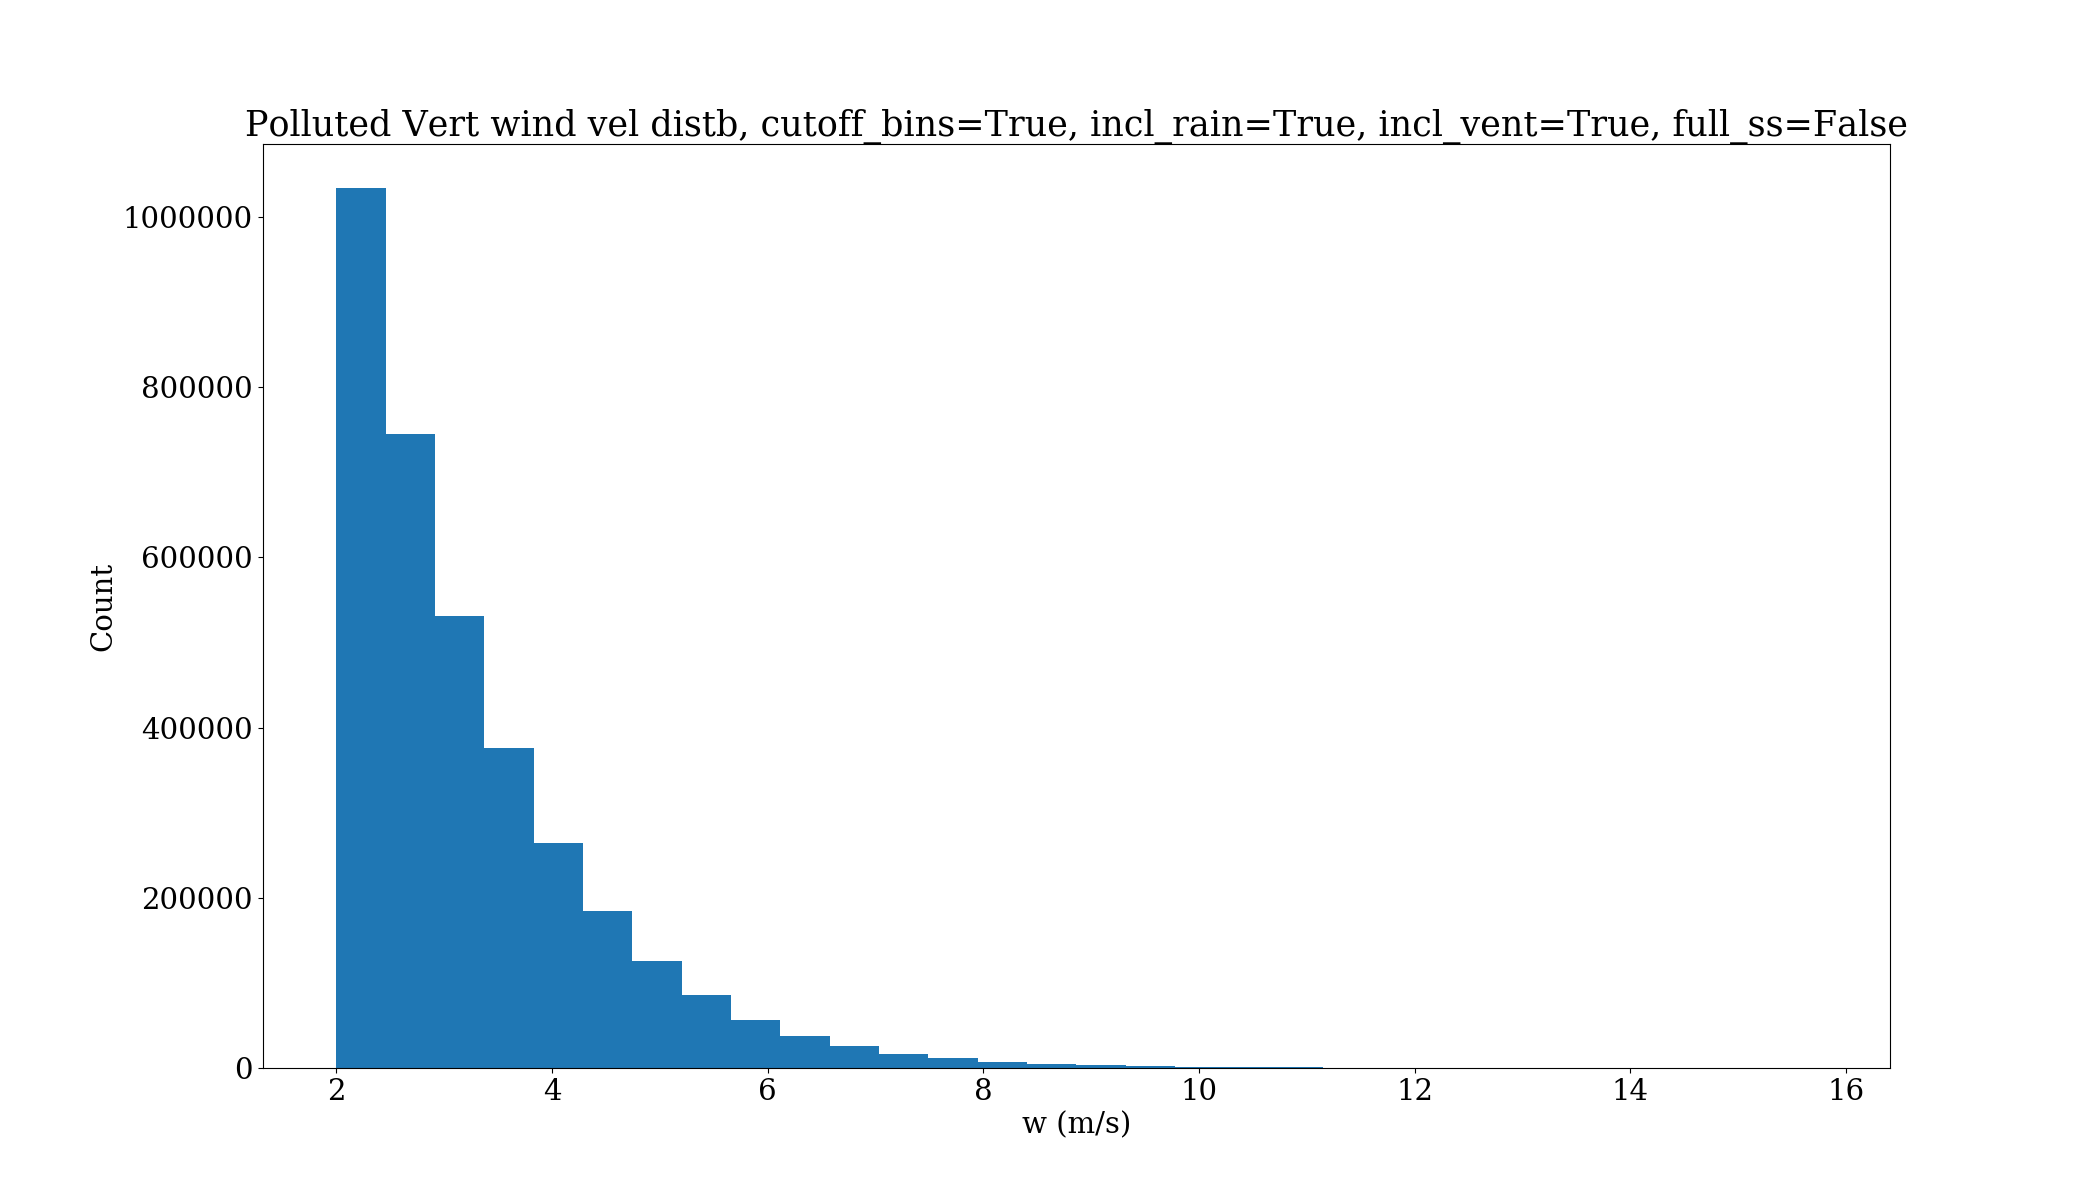
\includegraphics[width=\textwidth]{revmywrf/v9_w_hist_Polluted_figure.png}
		\caption{Polluted case.}
		\label{wrfwhistpoll}
	\end{subfigure}
	\caption{Vertical wind velocity distribution in WRF simulation using filtering criteria described in the text.}
	\label{wrfwhist}
\end{figure}
\begin{figure}[ht]
    \centering
    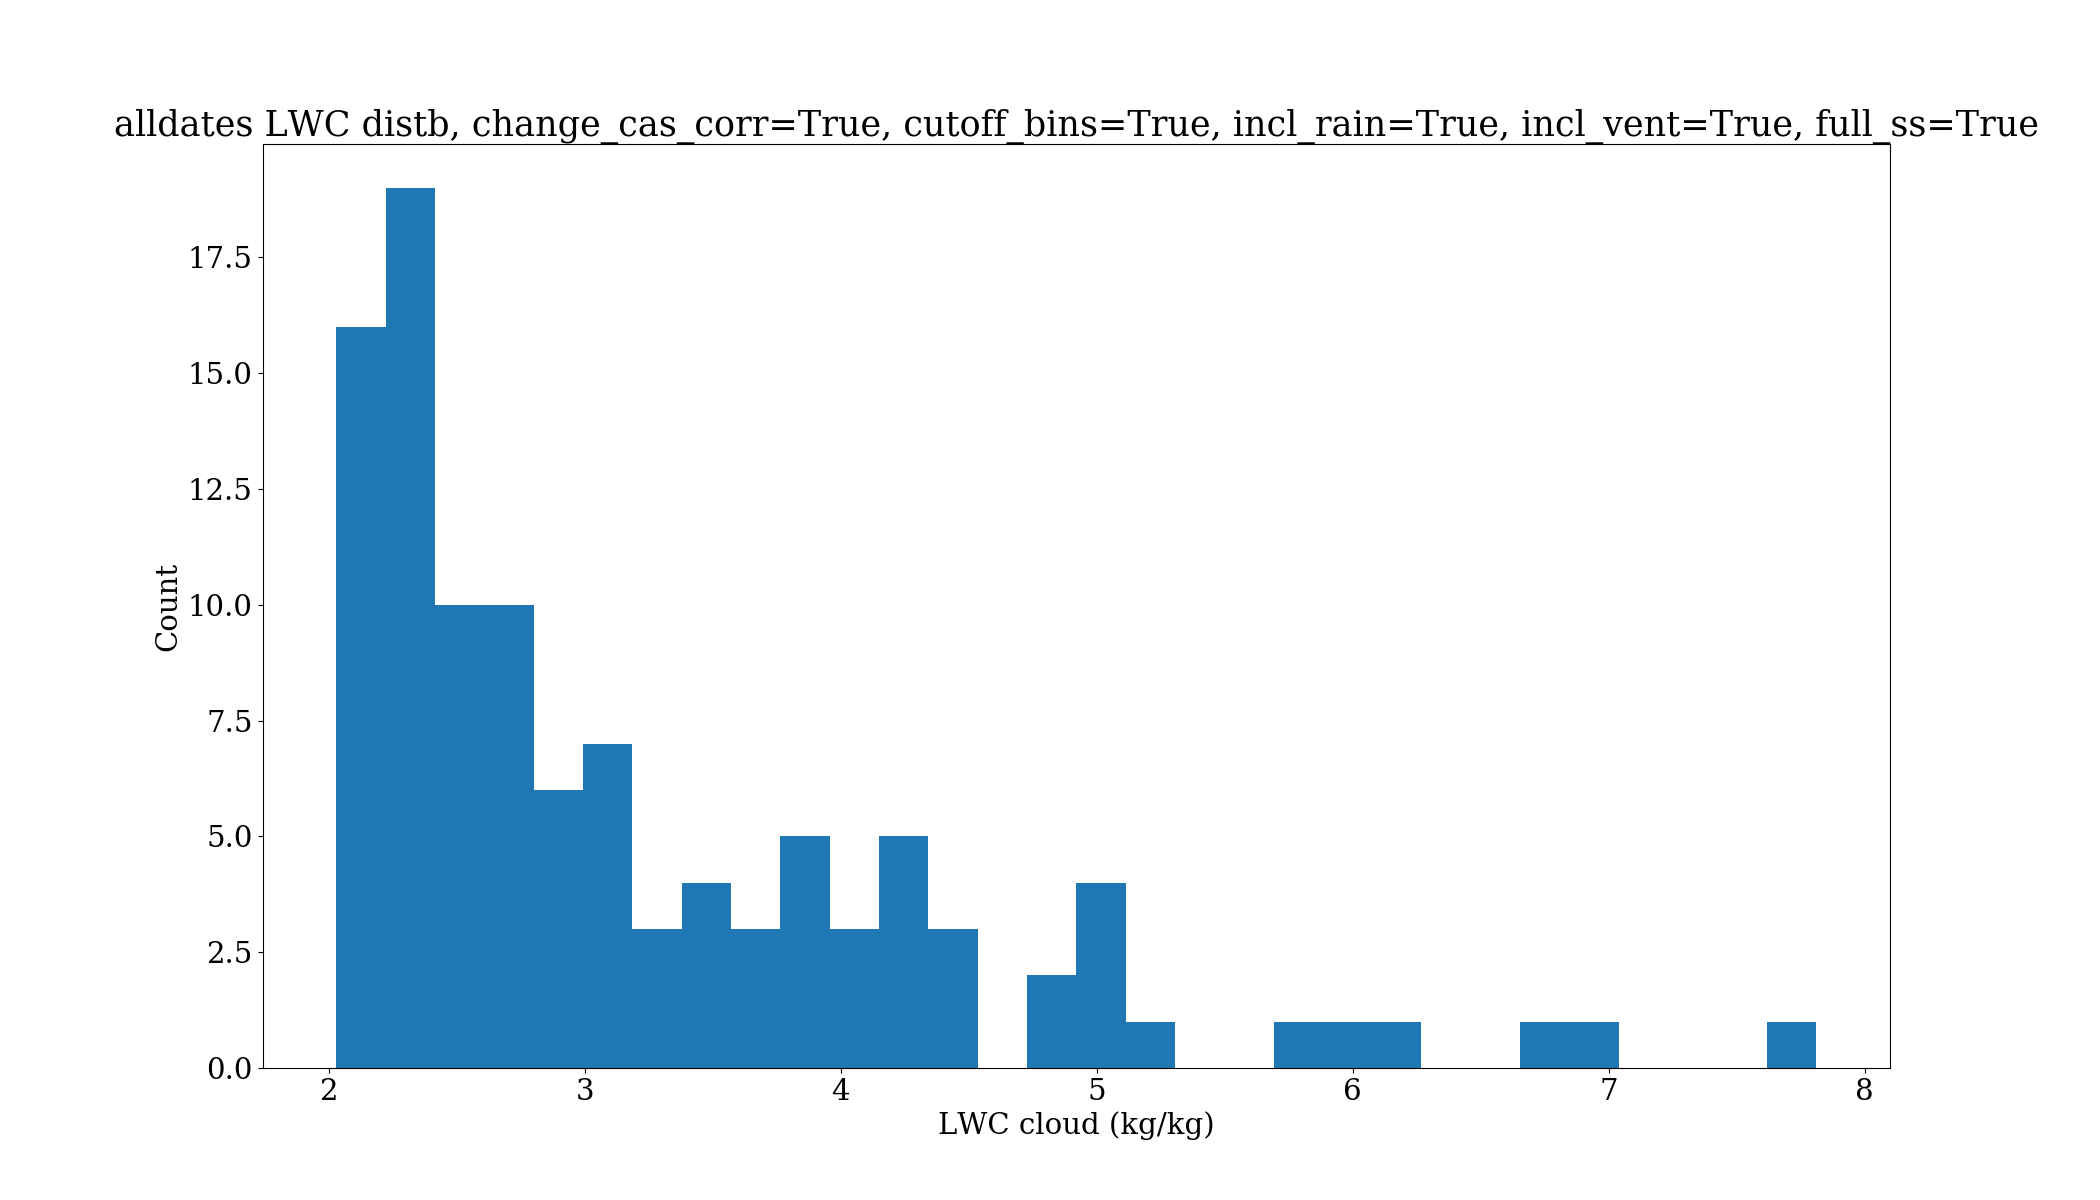
\includegraphics[width=9cm]{revhalo/v24_w_hist_cas_alldates_figure.png}
    \caption{Vertical wind velocity distribution from HALO field campaign (all flight dates). Using filtering criteria outlined in section 2.}
    \label{halowhist}
\end{figure}
\begin{figure}[ht]
    \centering
    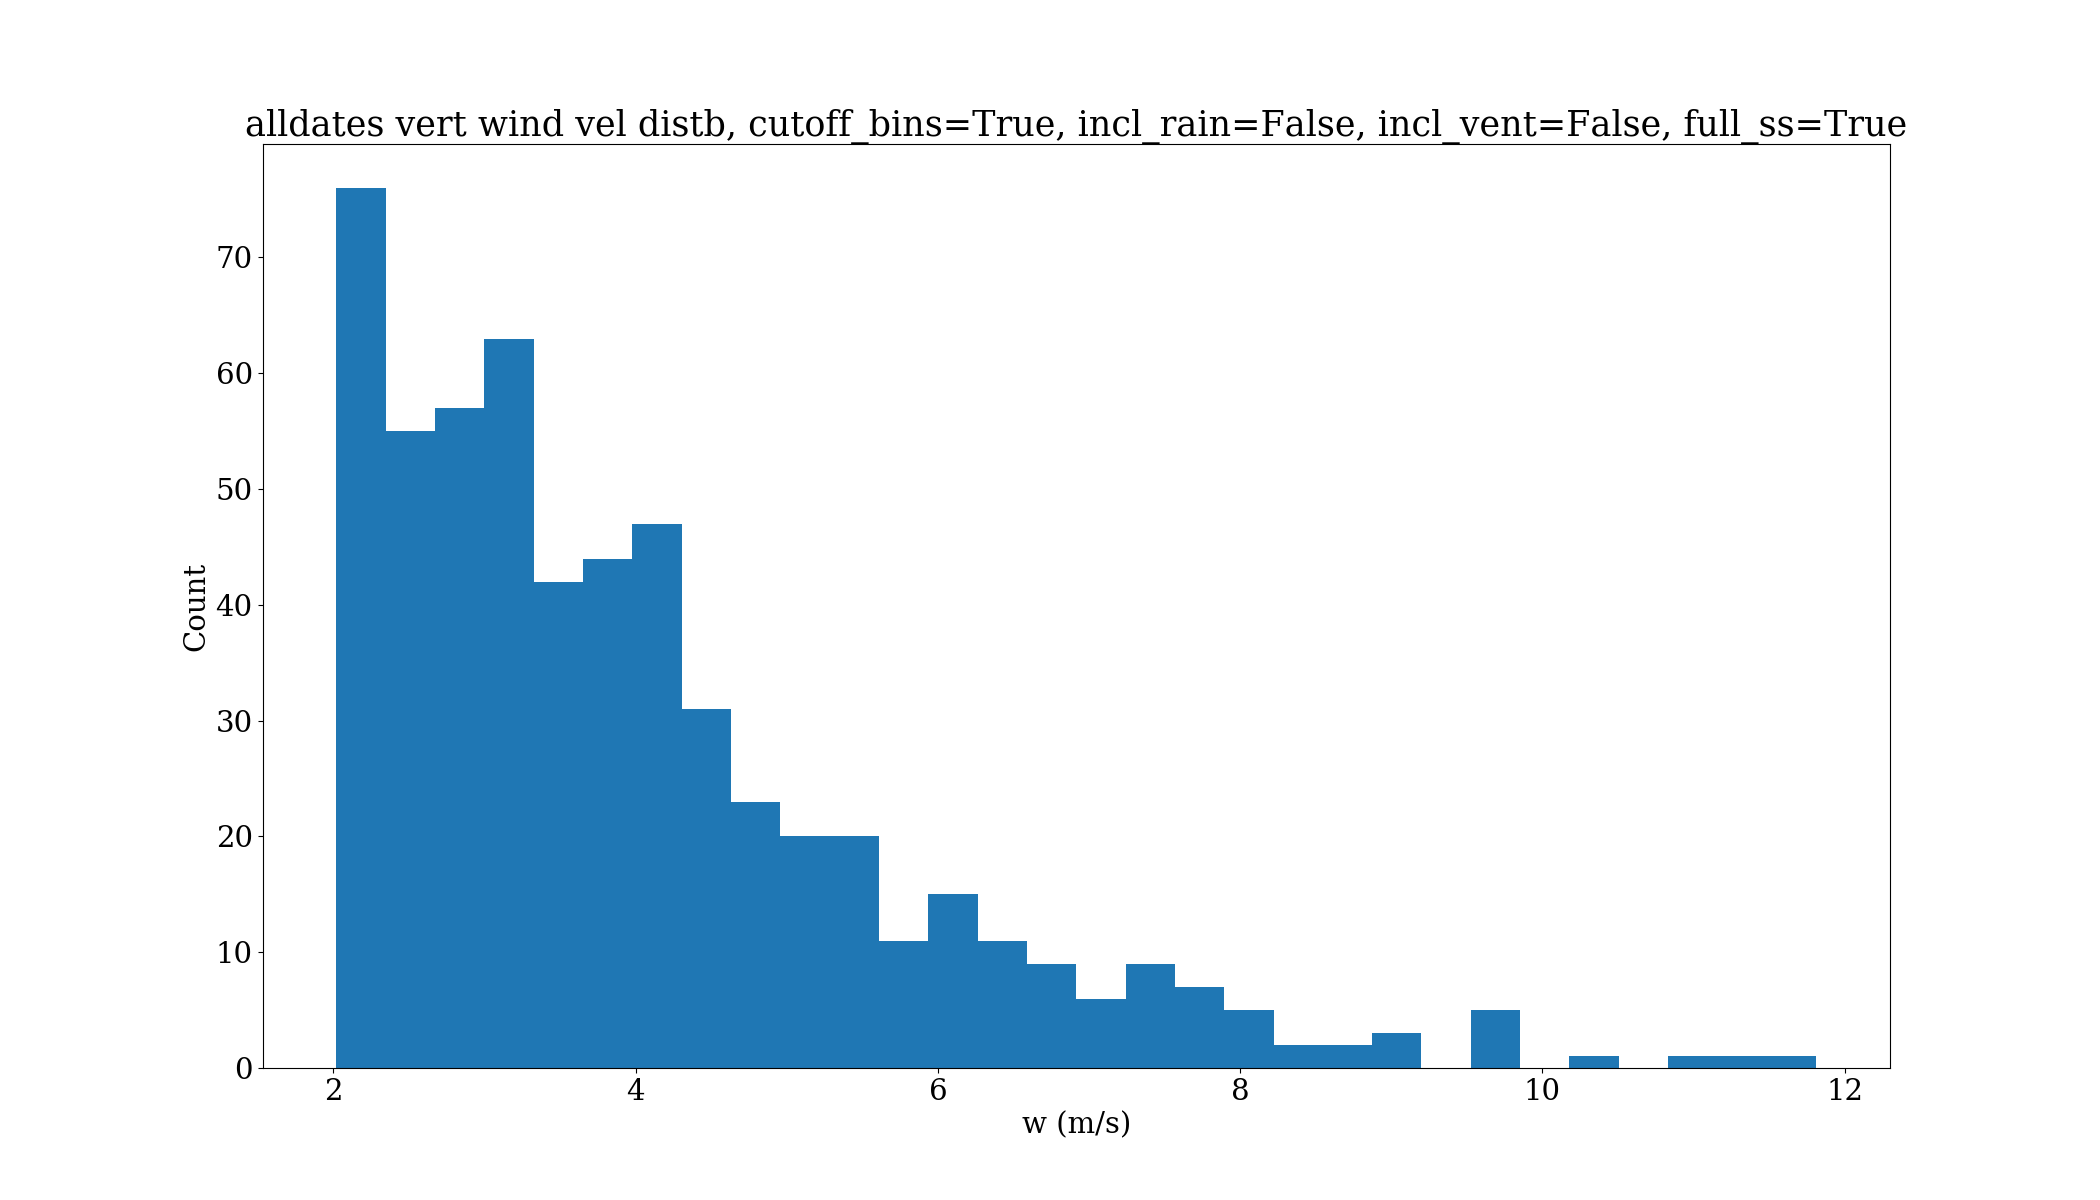
\includegraphics[width=9cm]{revcaipeex/v10_w_hist_alldates_figure.png}
    \caption{Vertical wind velocity distribution from CAIPEEX field campaign (all flight dates). Using filtering criteria outlined in section 2, but not including rain drops or ventilation corrections due to lack of data.}
    \label{caipeexwhist}
\end{figure}

\section{Environmental conditions - simulation vs experiment}
- under above filtering criteria: lwc distbs for wrf (FIG), halo (FIG) and caipeex (FIG)
- for clear-sky points below freezing level: aero psds for halo vs wrf (FIG) and caipeex vs wrf (FIG)

\subsection{LWC}

\begin{figure}[ht]
	\centering
	\begin{subfigure}{0.7\textwidth}
		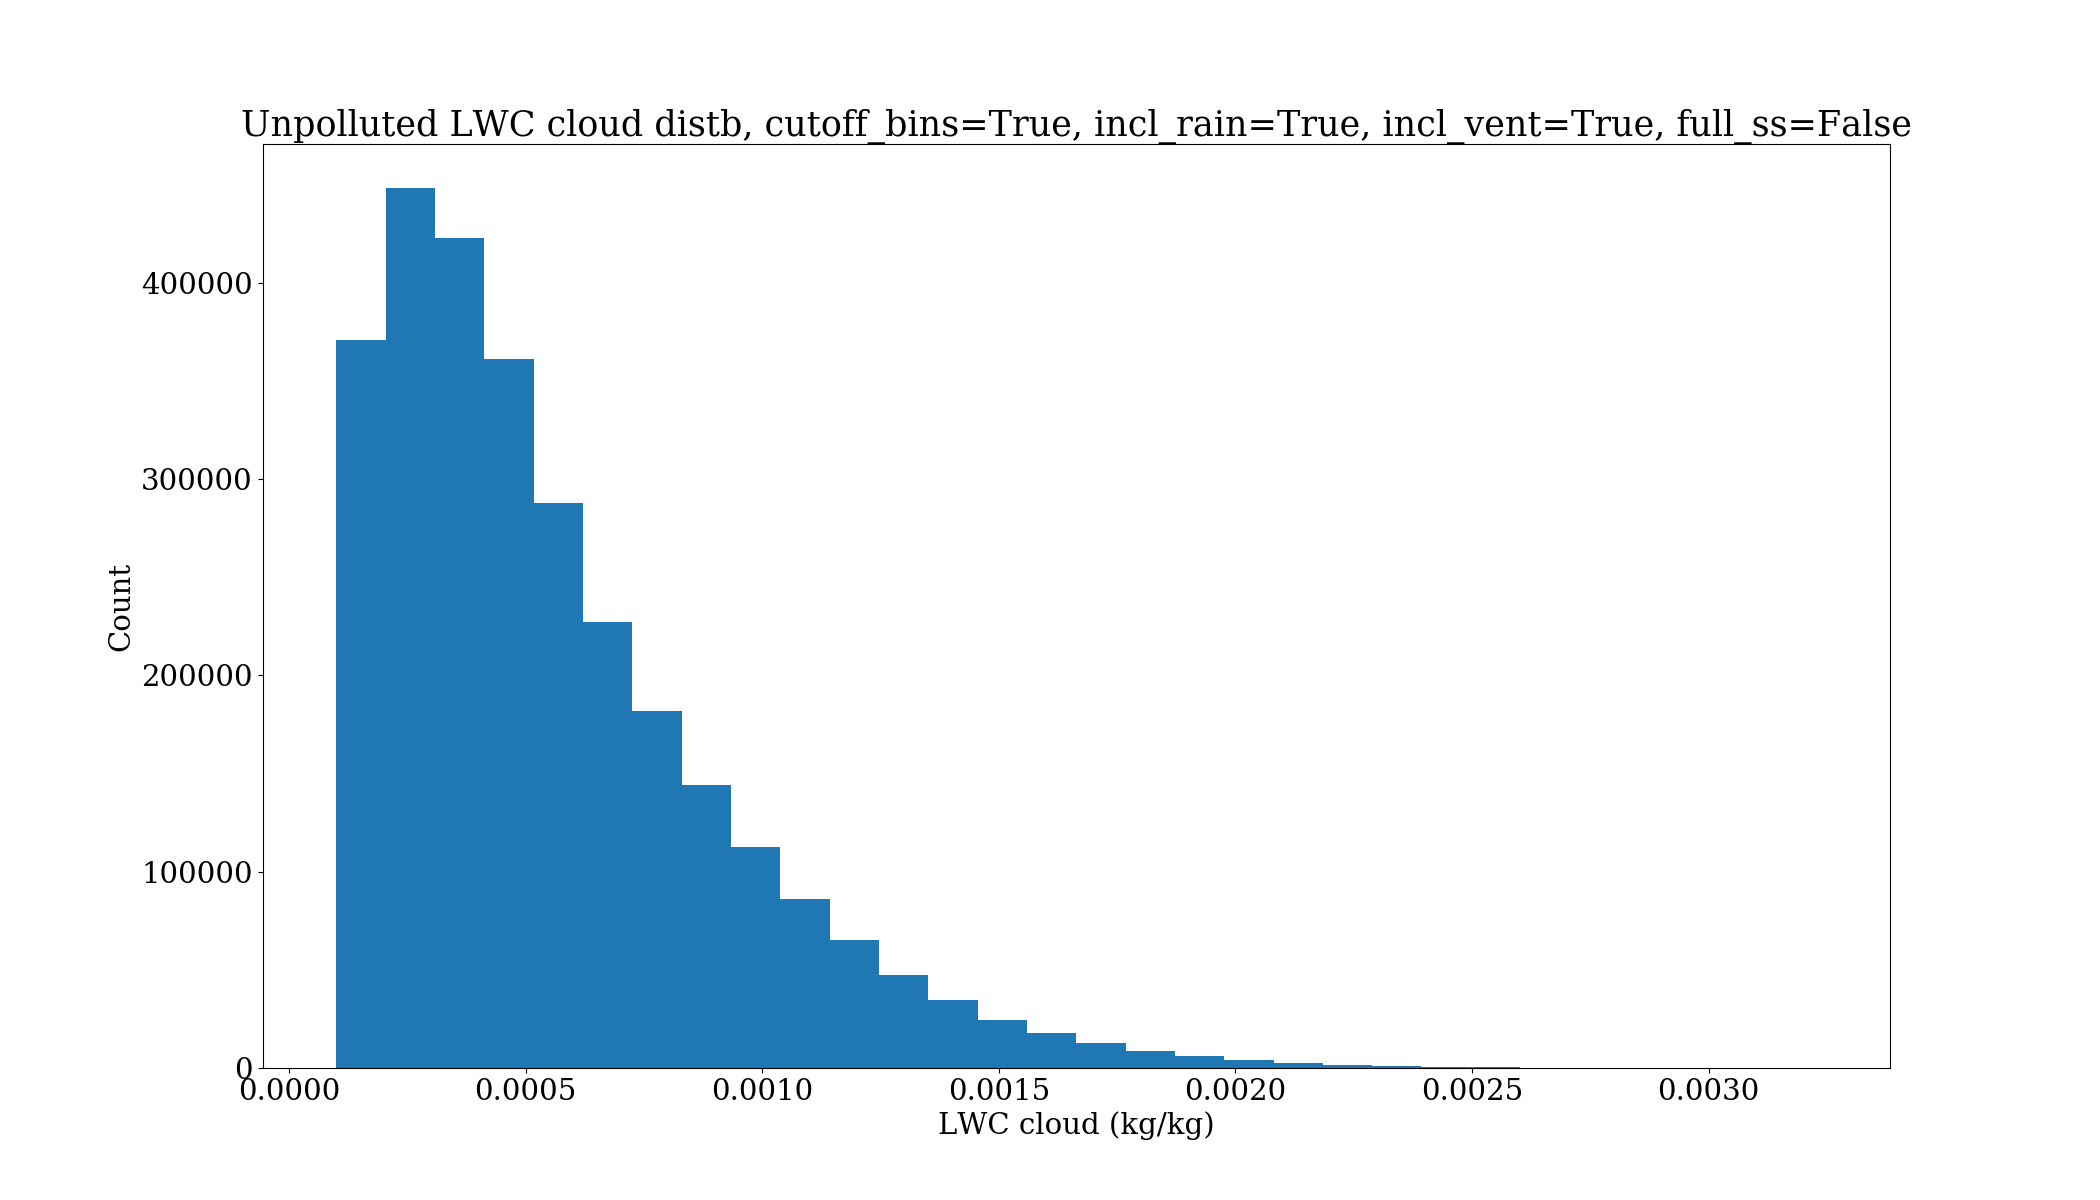
\includegraphics[width=\textwidth]{revmywrf/v9_lwc_hist_Unpolluted_figure.png}
		\caption{Unpolluted case.}
		\label{wrflwchistunpoll}
	\end{subfigure}
	\begin{subfigure}{0.7\textwidth}
		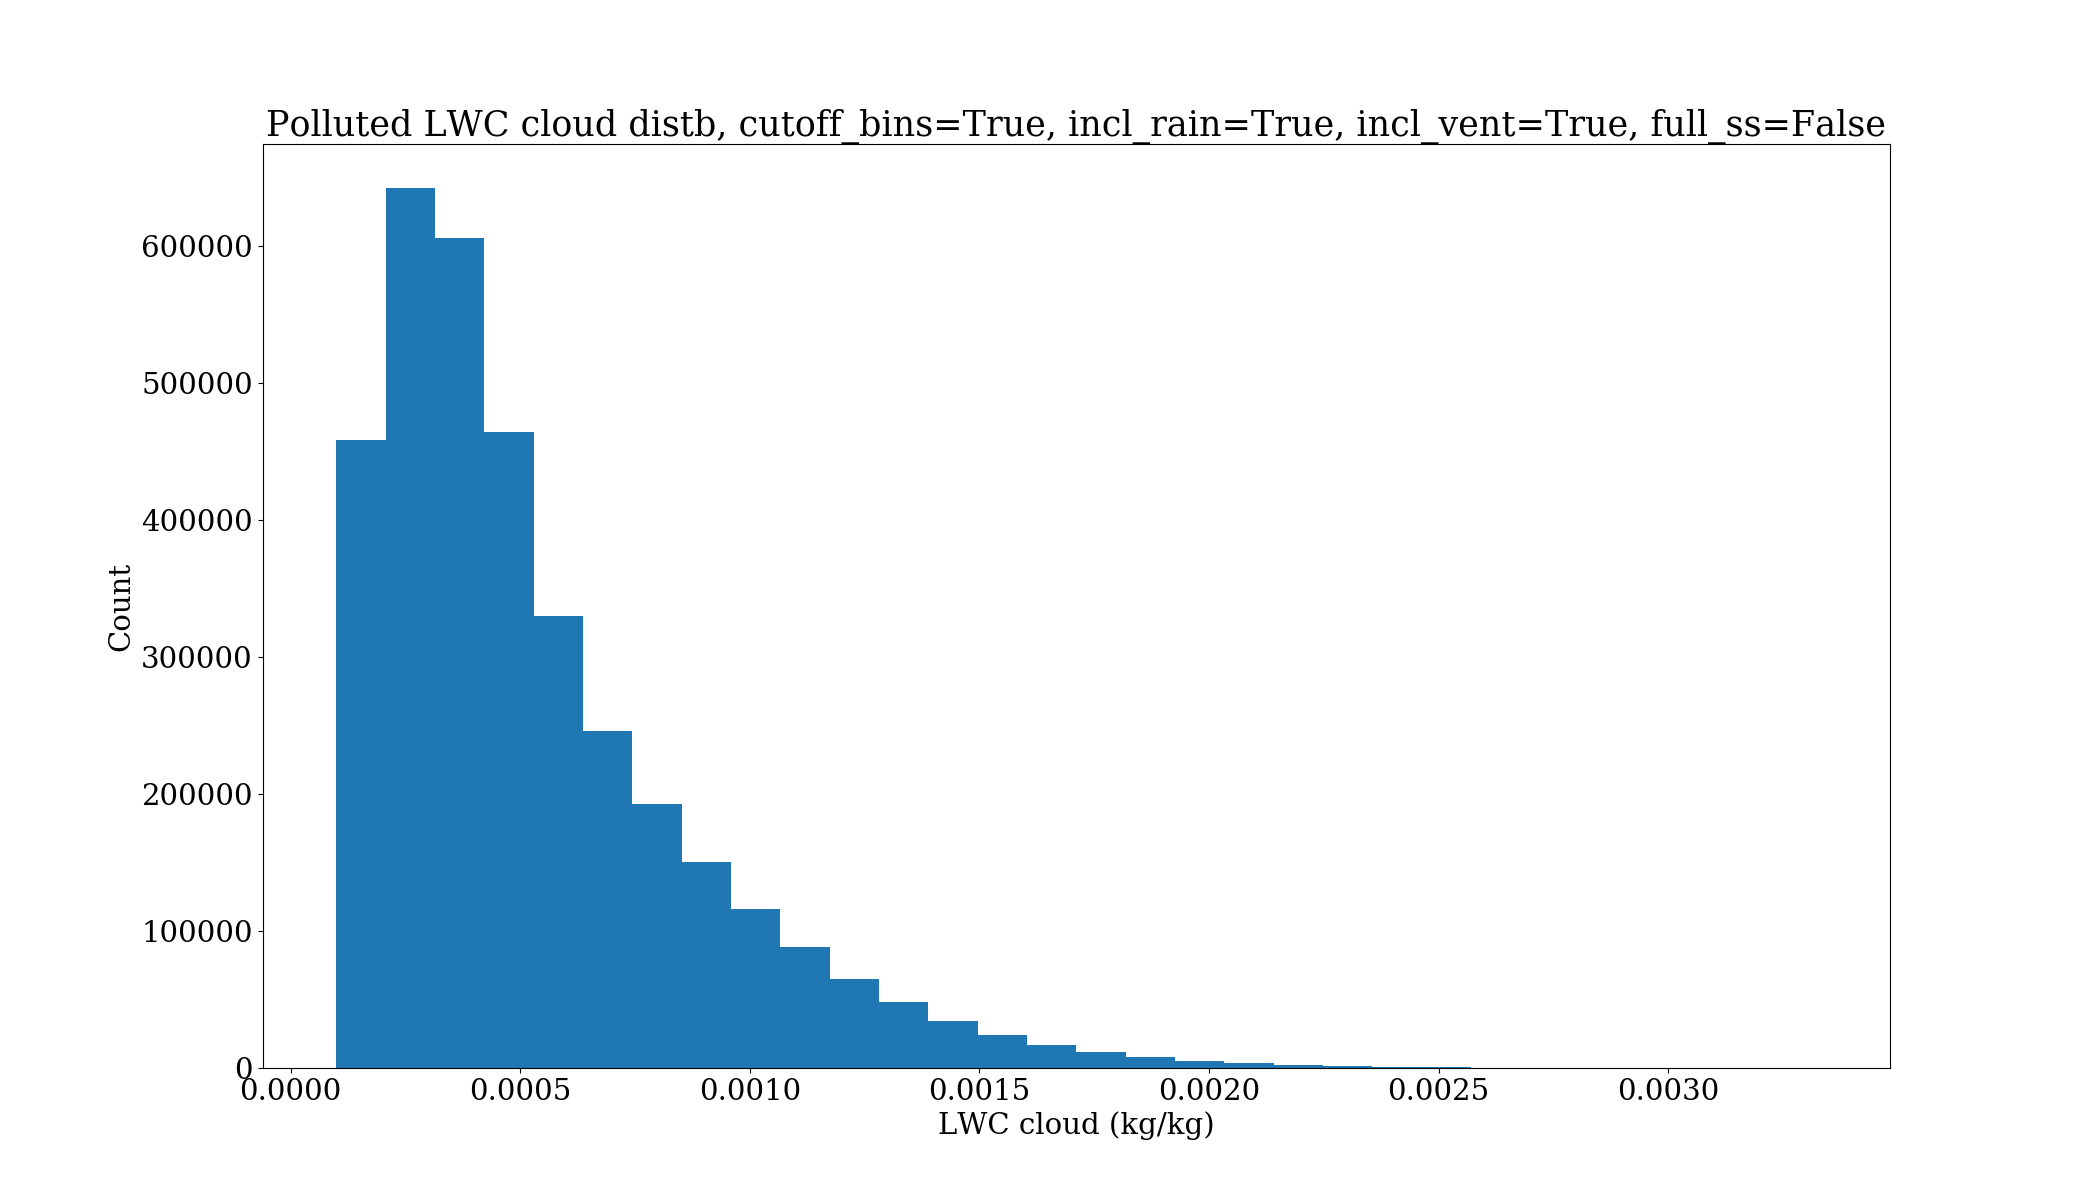
\includegraphics[width=\textwidth]{revmywrf/v9_lwc_hist_Polluted_figure.png}
		\caption{Polluted case.}
		\label{wrflwchistpoll}
	\end{subfigure}
	\caption{Cloud LWC distribution in WRF simulation using filtering criteria described in the text.}
	\label{wrflwchist}
\end{figure}
\begin{figure}[ht]
    \centering
    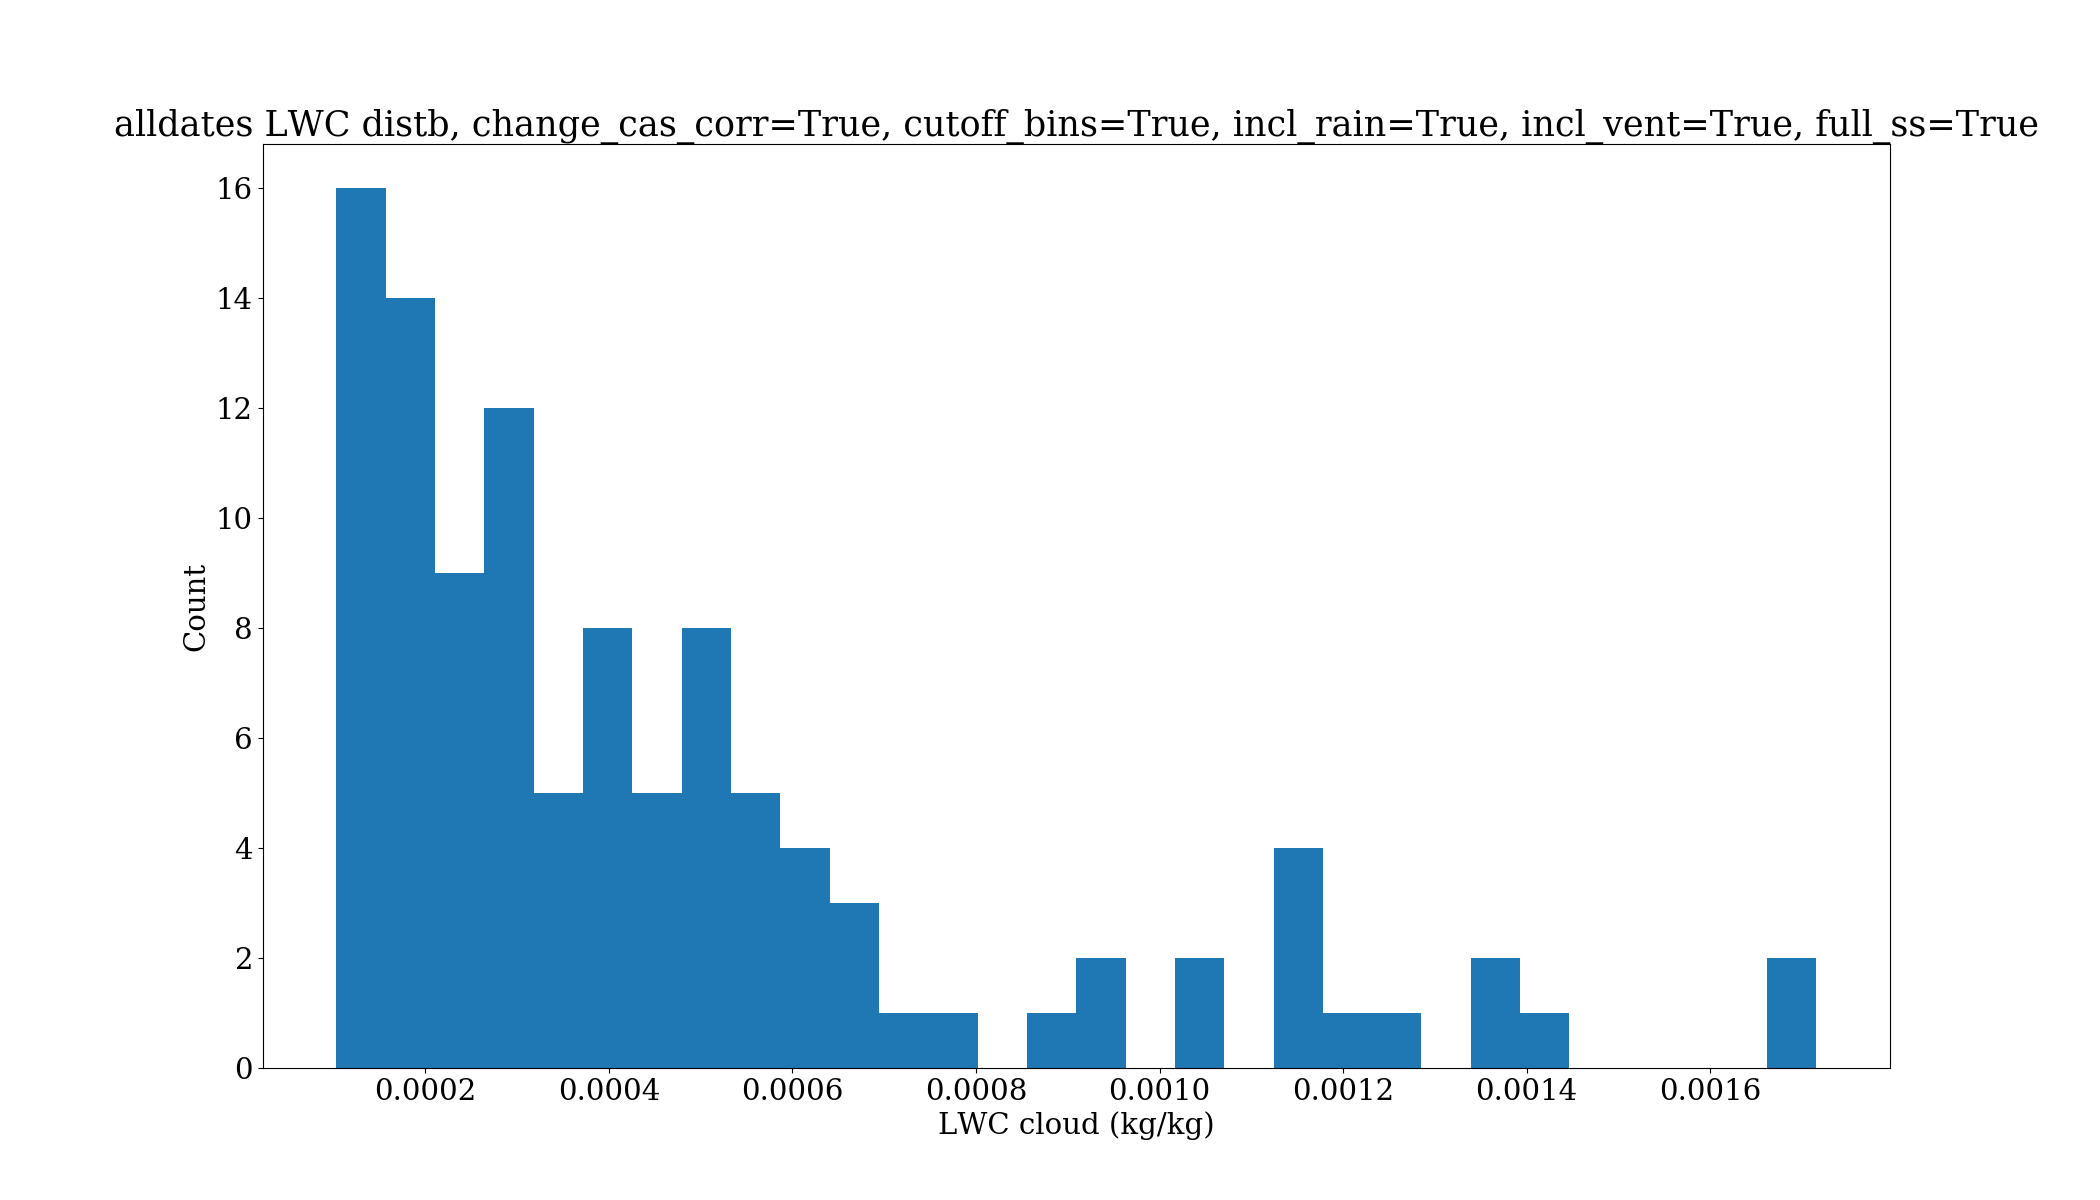
\includegraphics[width=9cm]{revhalo/v24_lwc_hist_cas_alldates_figure.png}
    \caption{Cloud LWC distribution from HALO field campaign (all flight dates). Using filtering criteria outlined in section 2.}
    \label{halolwchist}
\end{figure}
\begin{figure}[ht]
    \centering
    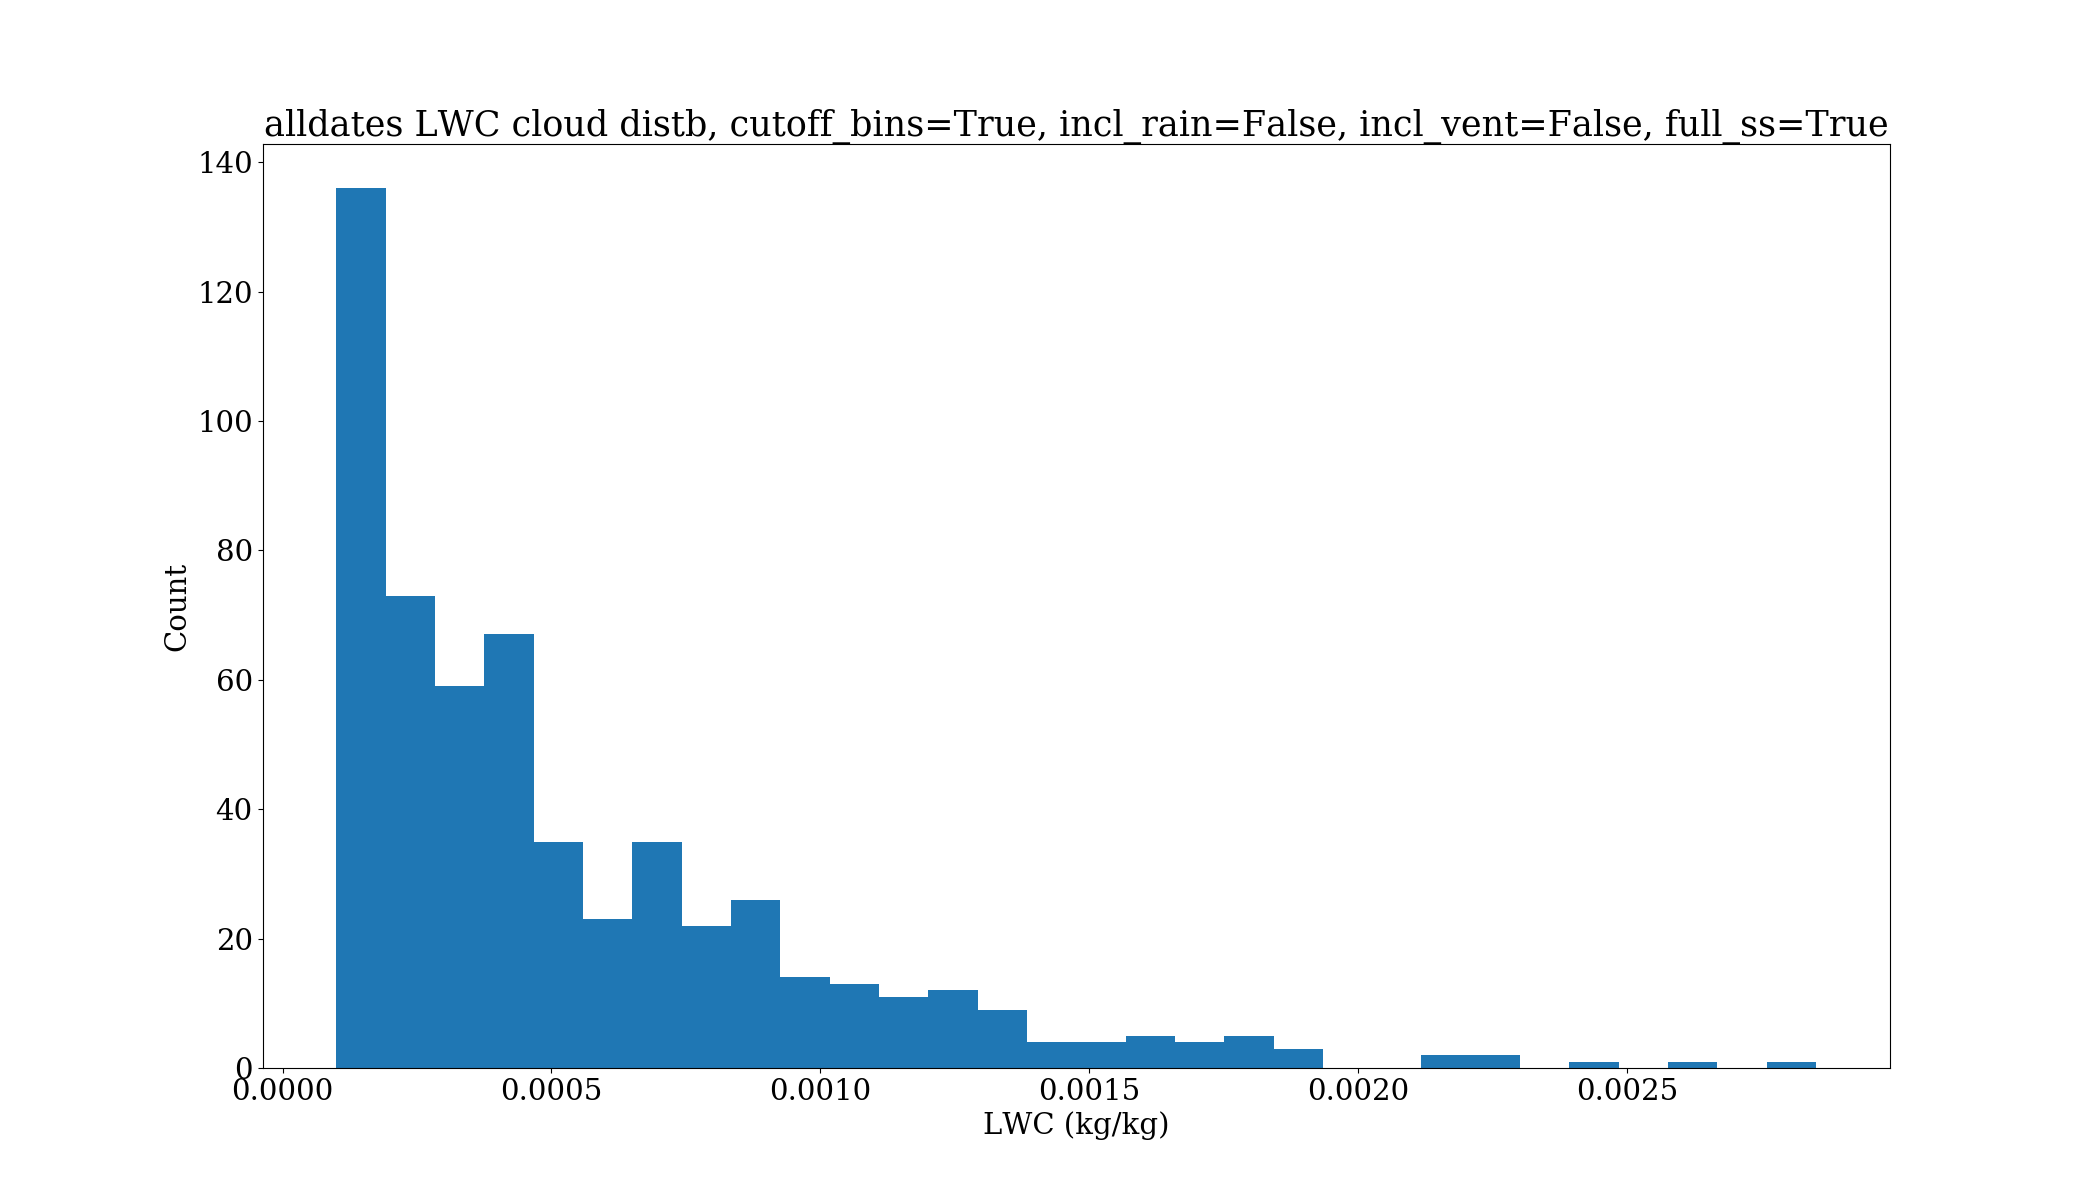
\includegraphics[width=9cm]{revcaipeex/v10_lwc_hist_alldates_figure.png}
    \caption{Cloud LWC distribution from CAIPEEX field campaign (all flight dates). Using filtering criteria outlined in section 2, but not including rain drops or ventilation corrections due to lack of data.}
    \label{caipeexlwchist}
\end{figure}

\subsection{Aerosol PSD}
\begin{figure}[ht]
    \centering
    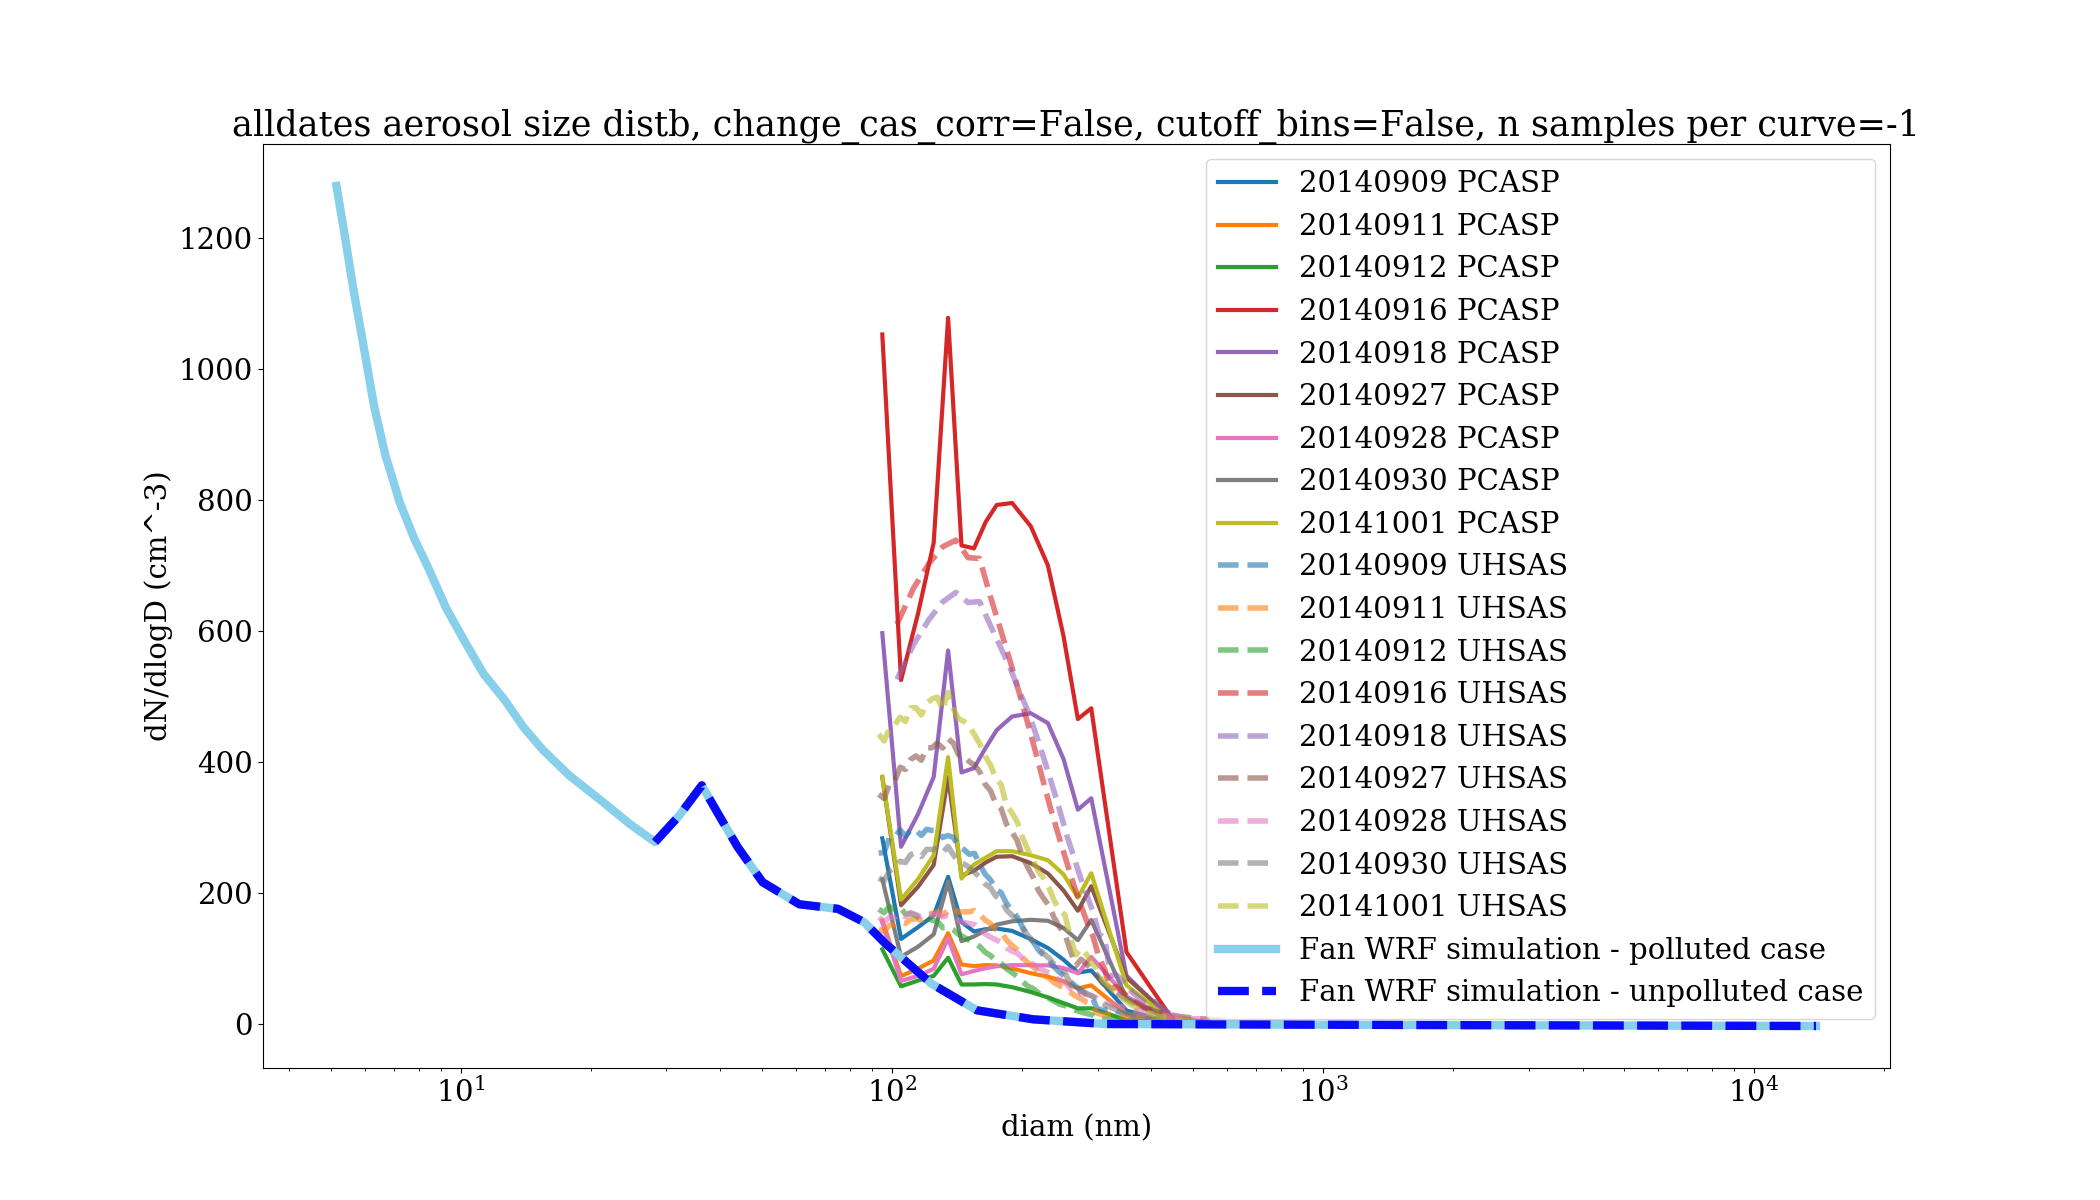
\includegraphics[width=9cm]{revhalo/v1_aero_size_distb_alldates_figure.png}
    \caption{Aerosol particle size distribution from HALO field campaign (all flight dates), compared to initial distribution in boundary layer for WRF simulation. Using clear sky points (LWC $\lt$ 1e-5) below the freezing level.}
    \label{haloasdhist}
\end{figure}
\begin{figure}[ht]
    \centering
    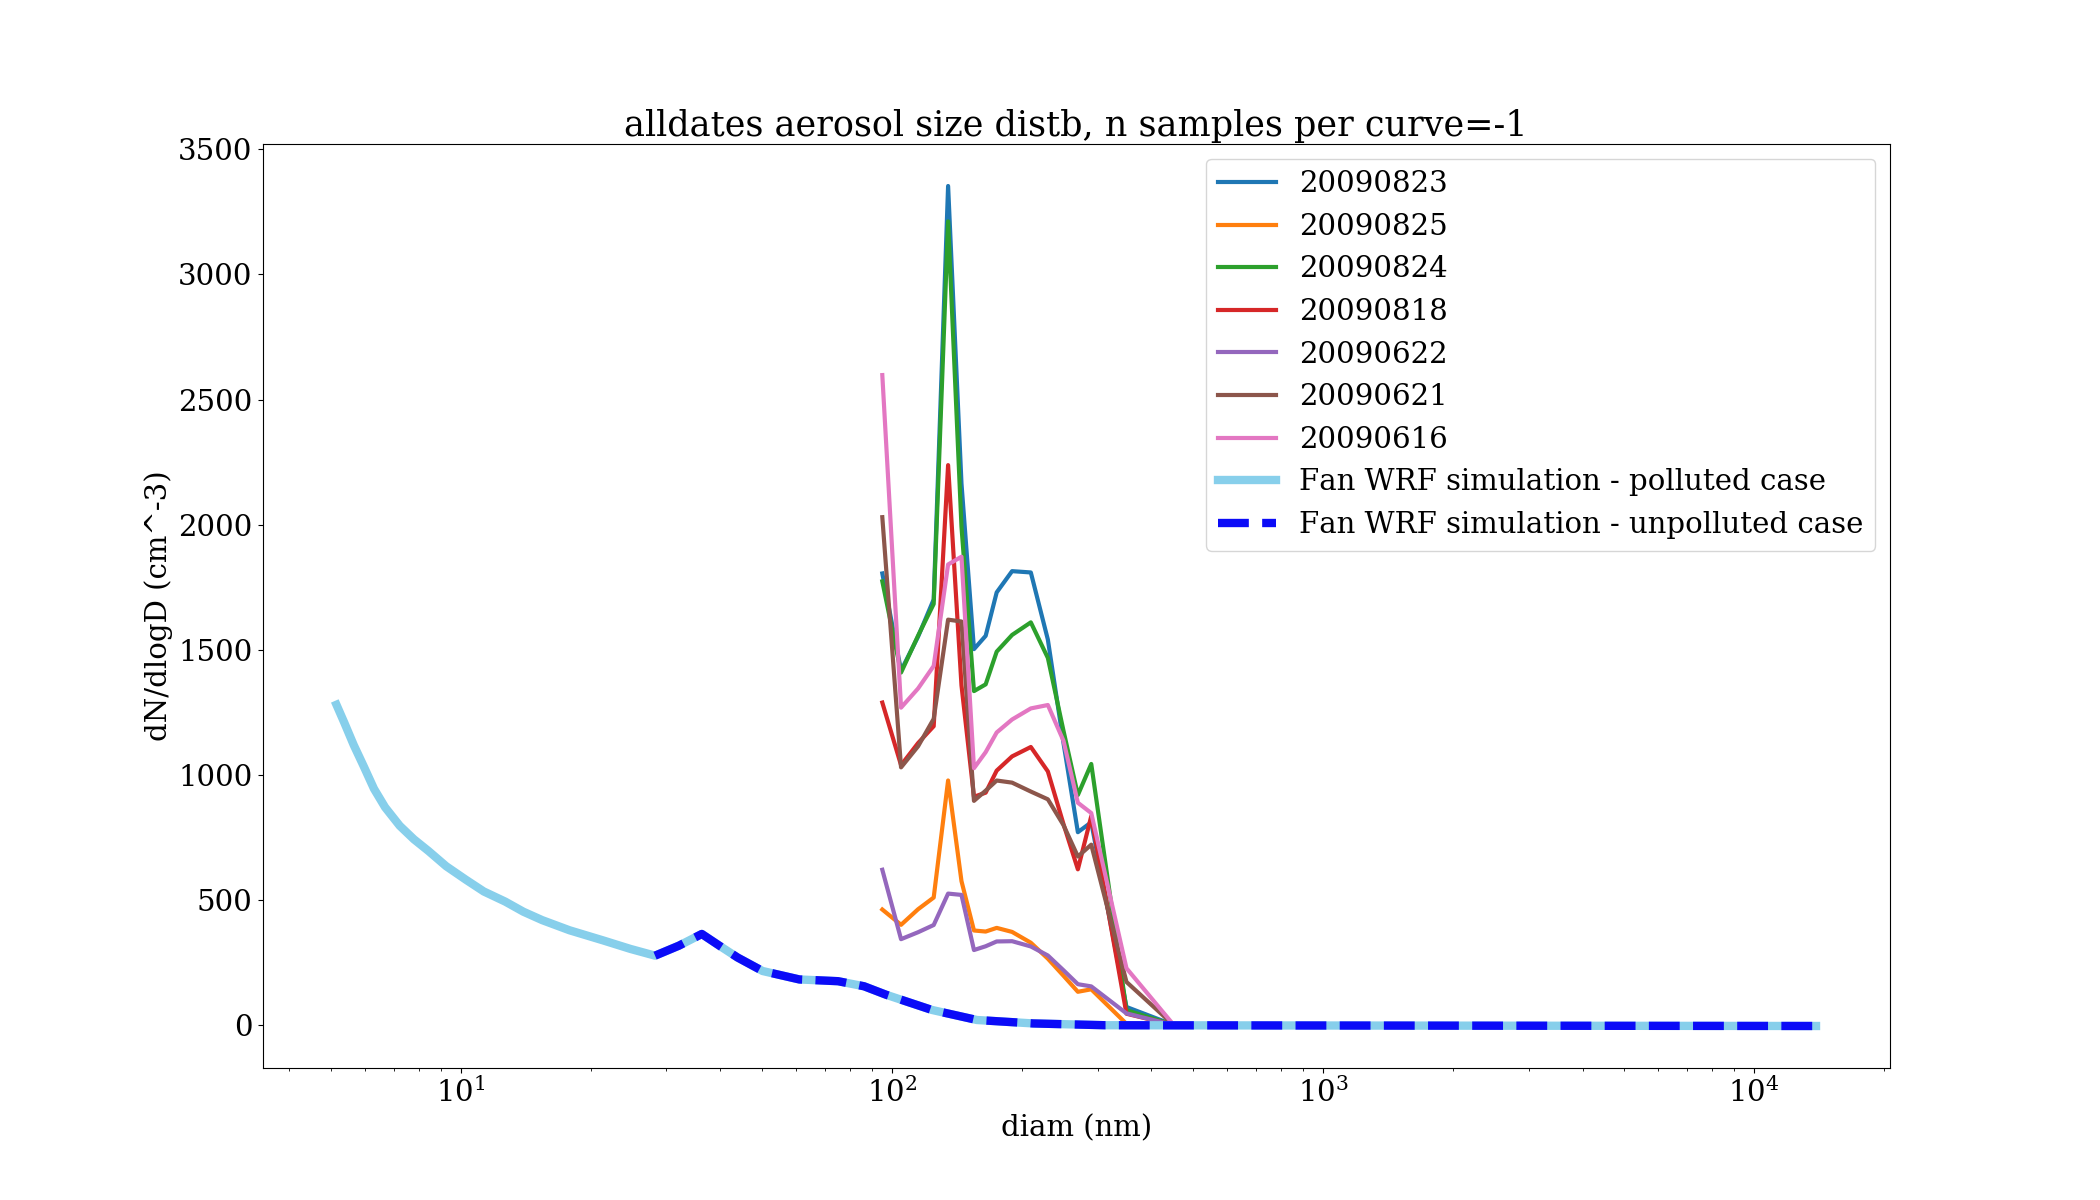
\includegraphics[width=9cm]{revcaipeex/v1_aero_size_distb_alldates_figure.png}
    \caption{Aerosol particle size distribution from CAIPEEX field campaign (all flight dates), compared to initial distribution in boundary layer for WRF simulation. Using clear sky points (LWC $\lt$ 1e-5) below the freezing level.}
    \label{caipeexasdhist}
\end{figure}

\section{Further discussion / conclusions}

\section{Figures to include in supplementary info}
\begin{itemize}
	\item all figures without lower bin cutoffs
	\item all figures without corrections from including raindrops / ventilation factors
\end{itemize}
\section{TODO / remaining questions}
\begin{itemize}
	\item in code: optimize HALO instrument time offsets
	\item error analysis for experimental data
	\item look into commensurate binning in simulation / experiment comparisons?
	\item analytical justification for why actual and QSS supersaturation is still in linear relation
	\item expt vs model cloud/rain droplet size boundary
\end{itemize}
This is a reference \cite{Fan2018}.
%\begin{figure}[h]
%    \centering
%    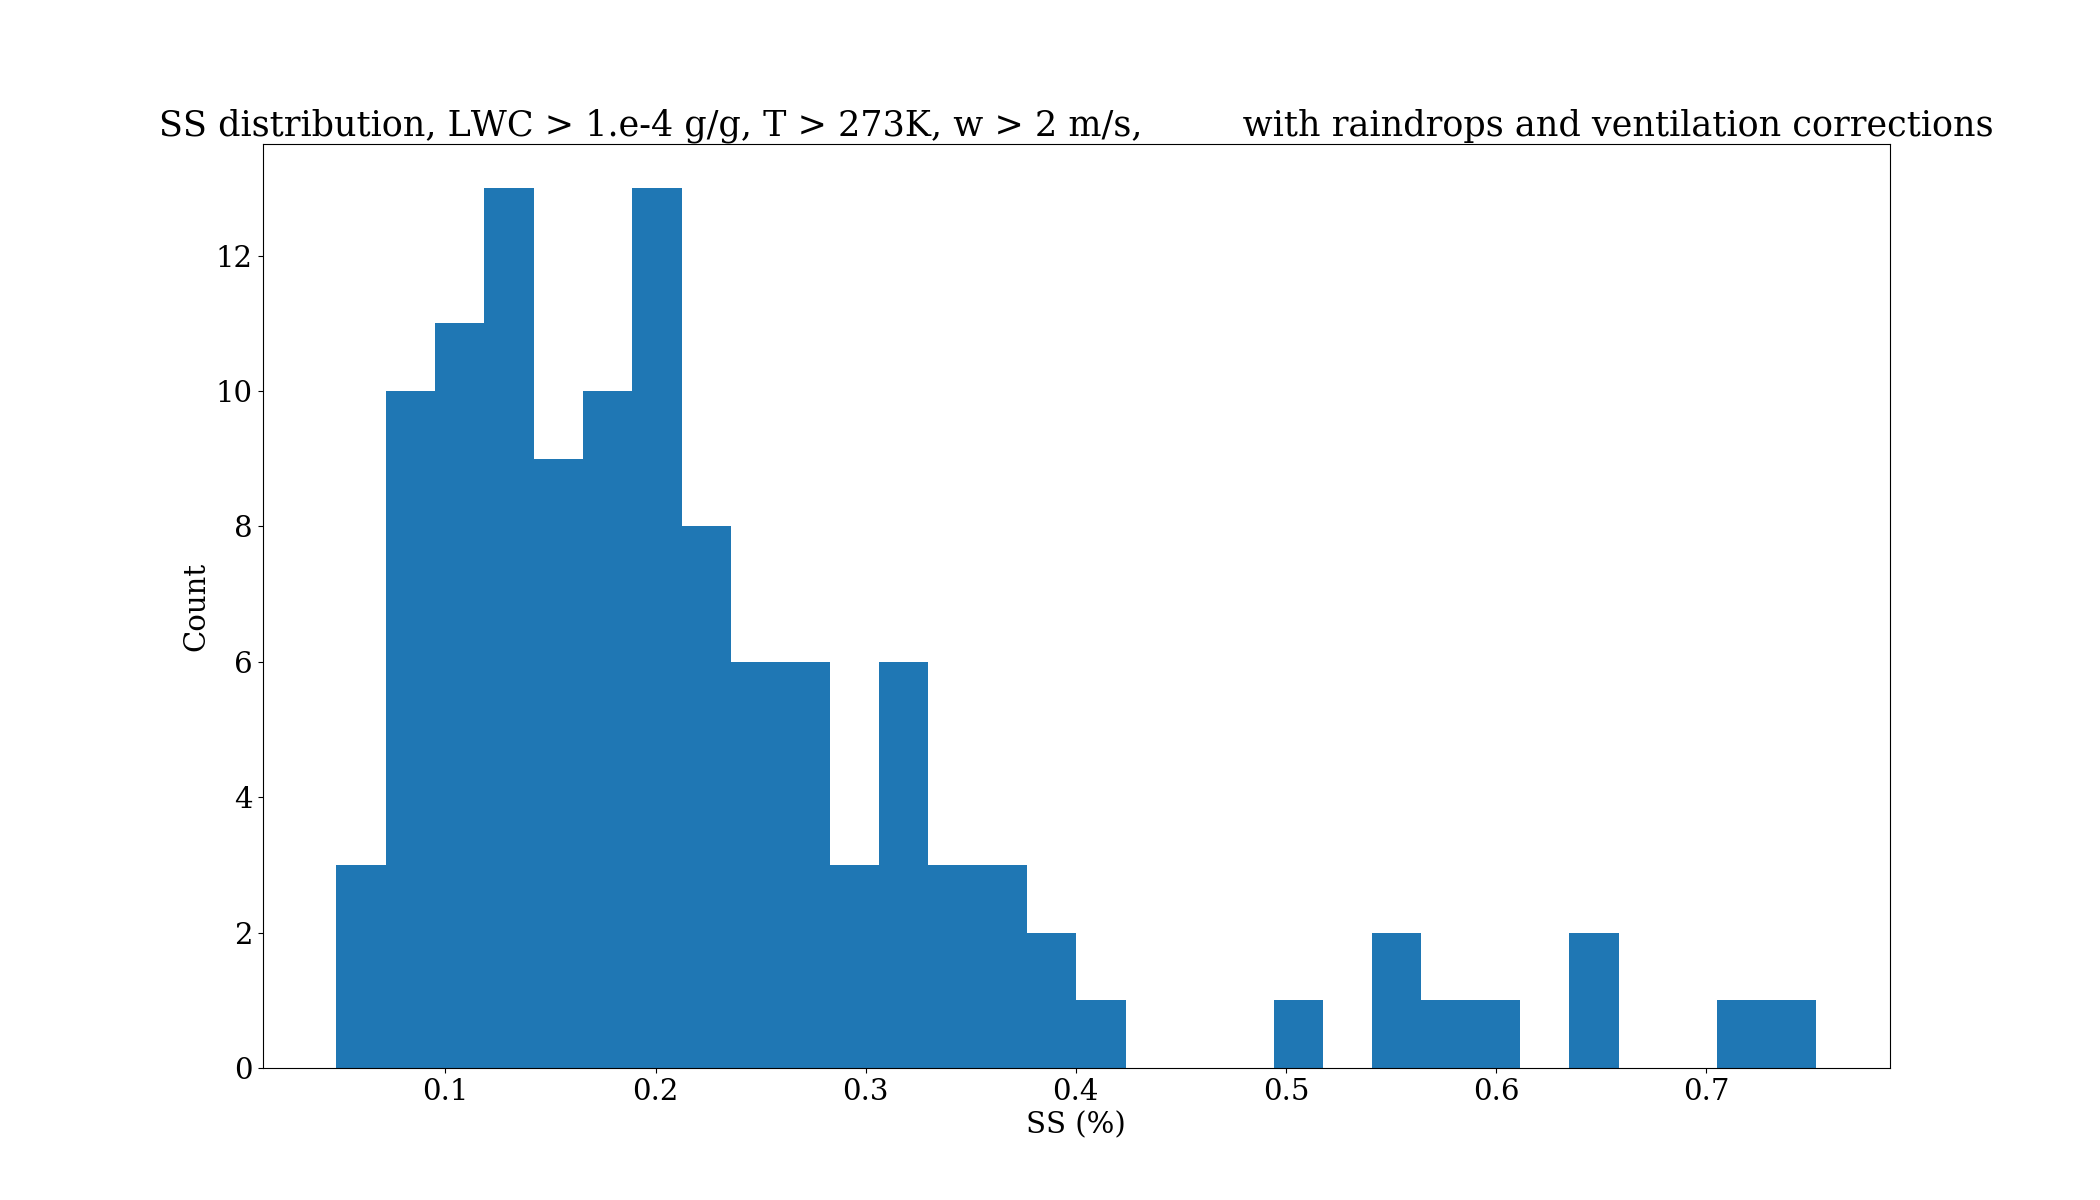
\includegraphics[width=9cm]{halo/v3_ss_with_cip_from_cas_alldates_figure.png}
%    \caption{}
%    \label{fig:fig_label}
%\end{figure}

\bibliography{refs}
\bibliographystyle{ieeetr}
\end{document}



